% Outline: 8
\chapter{可信强化学习}
\label{chap:rl-trustworthy}

前几章评价一个策略时，默认问题几乎只有一个：它的期望回报有多高。这个标准在多数回合表现正常时足够好用，却回答不了一类更尖锐的问题——“出状况的那几次怎么办”。考虑一台导航机器人：它在大多数回合很快到达终点，只在少数回合严重延误。平均到达时间即使很短，也把顺利回合和糟糕回合混在了一起，无法说明这些延误是否可以承受。更麻烦的是，训练时假设的环境与部署时未必相同：地面变湿时，原来学到的制动规律可能整体失效；而在机器人上启用一个会在危急时刻接管的紧急保护器后，“没有碰撞”又可能只是保护器替换了危险动作的结果，并不能说明原策略本身可靠。于是部署判断需要回答两个层次不同的问题：第一，我们究竟希望机器人满足什么行为要求——是平均表现好，还是最差的回合也不能太糟，是湿滑地面也要能用，还是任何时候都不许碰撞；第二，手头的证据——无论是有限的试验记录还是基于模型的证明——是否足以支持这些要求。前者是在规定“什么算合格”，后者是在核查“凭什么相信它合格”。

本章沿用第~\ref{chap:rl-overview}~章的策略与轨迹，以及第~\ref{chap:rl-planning}、\ref{chap:rl-learning}~章的规划和学习工具。回答第一个问题时，三种要求分别从三个不同的环节收紧决策：风险敏感决策改变的是随机后果的评价方式，例如不再只看平均损失，而比较最差那部分回合的损失；鲁棒决策改变的是环境范围，要求同一策略在允许的环境变化下都维持表现；安全约束改变的是可行策略集合，把不满足成本预算或边界要求的策略直接排除。三者改动的对象不同，可以组合使用，但并无必须依次采用的演进顺序。求出候选策略后，第二个问题——证据——才登场：此时评价一个已经冻结的策略、评价一条固定学习规则重复训练出的多个策略、以及评价一个带保护器的完整执行系统，是三种随机性来源不同、结论也不同的取证任务，必须分开处理。

图~\ref{fig:rl-trustworthy-map}~将三类要求放在相同的任务设定下。各分支先给出要维护的性质和求解方法，再由验证过程检查候选方案；方案比较中的保证只在相应运行条件和证据范围内成立。

\begin{figure*}[t]
  \centering
  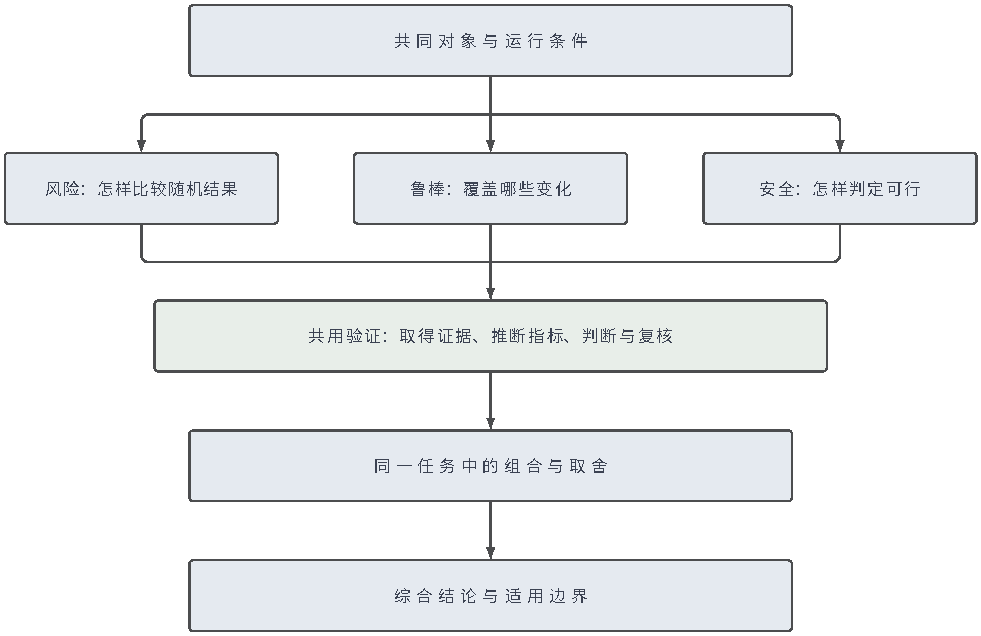
\includegraphics[width=166.169mm]{figures/10-reinforcement-learning/03-task-expansion-and-trustworthiness/tikz/rl-trustworthy-map.pdf}
  \caption{可信强化学习的章内关系。共同设定固定决策对象和运行条件，三个分支提出行为要求与候选策略，验证过程据此判断组合方案。箭头表示模型、策略、验证记录与结论之间的依赖，不表示风险、鲁棒与安全必须依次执行；综合结论仍保留各分支的适用条件。}
  \label{fig:rl-trustworthy-map}
\end{figure*}

% Outline: 8.1
\section{行为要求与保证对象}
\label{sec:rl-trustworthy-requirements}

要把上面三个要求讲清楚，先得学会做“只改一项条件”的受控比较——如果好几个因素同时变化，观察到的成功率改变就无法归因。仍考察从起点驶向终点的移动机器人。在相同的几何路线、初始位置与动力学下，比较不同速度控制策略诱导的到达时间分布，可以检查偶发严重延误；固定策略与目标，改变地面摩擦，可以检查制动距离。若环境不变，只把一块原本可以穿越的地带声明为危险区，改变的则是行为是否被允许的判定标准。最后，启用会替换危险动作的保护层，改变了实际执行机制。四种比较各自只改变一项条件，因而能够分别识别结果分布、环境变化、行为可行性和保护器的影响；一个总成功率无法区分这些影响。

离散导航示意沿用宽4、高3的网格、起点$(1,1)$、终点$(4,3)$和障碍$(2,2)$。数值例子会分别声明采用基准滑移模型，还是把整段路线汇总为一次选择的教学模型；路线模型用于手算，不是随机网格的精确解。连续控制仍写作$\bm{x}_{t+1}=\bm{A}\bm{x}_t+\bm{B}\bm{u}_t+\bm{w}_t$，状态可以包含位置和速度；允许扰动$\bm{w}_t$的范围来自另行给定的运行条件，不能从动力学方程本身读出。

在给出具体要求之前，先要统一描述“一次运行会产生什么、我们又能测量什么”，因为后面三类准则比较的正是这些不同的量。同一回合既可能效率高，也可能靠近过危险区，还可能发生碰撞；只用一个标量回报无法同时表达这些后果。下面先固定评价对象，再谈怎样用它们提要求。

\begin{definition}[回报、损失、成本与失败事件]
  \label{def:rl-trustworthy-objects}
  固定动态环境$\mathcal E$、观测与反馈机制和策略$\pi$，得到理论轨迹律$P_{\mathcal E}^\pi$；实际可取得的评价记录服从$P_{\mathrm{rec}}^\pi$。若损失含未记录状态，还须说明能否由这些记录识别损失的分布。记相应的轨迹样本空间为$\Omega_{\mathrm{traj}}$，其事件$\sigma$代数为$\mathcal F_{\mathrm{traj}}$（即我们能对其讨论“发生概率”的那些轨迹集合，例如“所有发生过碰撞的轨迹”构成的集合）。无限时域取$0\leq\gamma<1$，并要求下面的奖励和成本级数绝对可积；有界逐步奖励与成本足以满足这一条件。
  对轨迹$\tau=(s_0,a_0,r_0,s_1,\ldots)$，回报为
  $G(\tau)=\sum_{t\geq0}\gamma^t r_t$，目标$J(\pi)=\mathbb E_\pi G$不作归一化。
  损失$L(\tau)$表示需要抑制的后果，数值越大越差；它可以是累计延误，也可以是$-G$，但必须明确选择。
  安全成本$c_{i,t}\geq0$记录第$i$类危险暴露或损害，其累计量为
  $C_i(\tau)=\sum_{t\geq0}\gamma^t c_{i,t}$。
  失败事件$F_H\in\mathcal F_{\mathrm{traj}}$是轨迹空间中的可测事件，因而$F_H\subseteq\Omega_{\mathrm{traj}}$；例如，它可以表示前$H$次动作中至少碰撞一次。
  有限时域任务取正整数$H$，求和截至$H-1$，不折扣时直接使用有限和；其期望也要求相应累计量可积。
\end{definition}

导航任务中，奖励可以衡量到达效率，损失可以记录延误，成本可以累计靠近危险区的时间，失败事件可以定义为发生碰撞。优化方向也随对象而异：回报越大越好，损失和成本越小越好，事件概率则须低于给定阈值。同一次碰撞可以同时增加损失和成本，但成本能够区分事故次数或严重程度，事件指示量$\mathbf 1\{F_H\}$只记录是否发生；比较尾部损失还要问最差的一部分结果究竟有多严重。

有了这些量，就可以从三个互不替代的角度提要求。三者回答的问题分别是“随机结果怎样比较”“环境可以怎样变”“哪些行为根本不许做”。\term{风险准则}（risk criterion）规定怎样根据随机结果的分布比较策略，例如比较最差回合的延误，而非只比较均值。\term{鲁棒要求}（robustness requirement）规定同一策略必须应对哪些动力学、观测或动作执行机制的变化，例如摩擦的物理区间或传感器的误差范围。\term{安全约束}（safety constraint）规定哪些行为可行，例如成本不超过预算、碰撞概率低于阈值，或始终不离开允许状态集。这里的允许集合由任务规格、设备能力或模型误差界确定；算法负责在这些条件下求解，并不自行决定什么后果可以接受。

\term{可靠性}（reliability）在本章指指定对象在声明运行条件下持续满足要求的程度。这里需要特别区分“算法在优化什么”和“系统实际做到了什么”：算法采用了风险目标或安全约束，只说明它尝试优化什么，还没有说明交付对象实际满足什么。要把“可靠”从一个形容词变成可判断的结论，还需要统计或模型证据支撑。

同样说“这个策略可靠”，被评价的对象不同，结论的含义也完全不同，因此需要先锁定保证对象。表~\ref{tab:rl-trustworthy-guarantee-objects}~据此区分三种保证对象。策略冻结后，轨迹差异只来自环境与动作采样，重复运行相当于对同一随机机制重复抽样；重新训练时，还会加入训练记录的采集与回放次序、参数初始化和探索随机性的差异，两次训练可能得到两个不同的策略；保护层启用后，实际动作可能不同于策略提出的动作，碰撞记录所评价的便是策略与保护层的组合，而不是原策略本身。

\begin{table}[htbp]
  \centering
  \begin{tabularx}{\linewidth}{@{}>{\raggedright\arraybackslash}p{20mm}XXX@{}}
    \toprule
    保证对象 & 随机性来源 & 评价单位 & 要求作用时机 \\
    \midrule
    固定策略$\pi$ & 初态、转移、观测、动作采样 & 一个完整运行回合 & 策略冻结后的部署 \\
    学习规则 & 训练种子、训练样本、探索与优化 & 一次完整训练及其输出 & 训练中或输出策略上 \\
    策略与保护层 & 上述运行随机性，以及保护器所用状态估计、模型预测及动作执行的误差 & 实际执行系统的一回合 & 所有受保护执行时刻 \\
    \bottomrule
  \end{tabularx}
  \caption{保证对象决定抽样单位。每行还须固定初态分布、观测接口、时域、交互权限及其他参与者的范围，不能把训练曲线平稳等同于系统安全。}
  \label{tab:rl-trustworthy-guarantee-objects}
\end{table}

为了让“可靠”有可判定的含义，需要把运行范围写入协议：从哪些位置启动，摩擦允许怎样变化，传感器误差多大，能否主动试探，其他机器人按什么规则行动，以及保护器是否启用。后文的风险分布、鲁棒模型集合和安全可行集合都在这份协议下定义；改变协议，就可能改变原声明的真假。

协议还须区分两个极易混淆的百分数：行为概率与统计置信水平。前者描述系统本身多常出错，后者描述我们这套估计程序有多常给出正确结论。$p=\mathbb P_\pi(F_H)$表示策略在运行中多常失败；$1-\delta$表示反复采用取证与推断程序时，所得界覆盖真实$p$的比例要求。前者描述行为，后者描述推断程序。例如$p\leq0.01$是在限制失败概率，置信水平$0.95$是在限制程序的覆盖错误，两者不能交换。阈值、运行范围和允许的推断错误率须在验证前确定；根据结果反复修改标准，既改变行为声明，也可能破坏原有统计覆盖。

% Outline: 8.2
\section{风险敏感决策}
\label{sec:rl-trustworthy-risk}

从这一节起，先处理三个要求中的第一个：环境模型和运行范围都固定不变，只比较其中的随机后果。即便环境的概率规律完全已知且保持不变，策略的随机化、初态和转移的随机性也会让每一回合的损失不同；期望回报准则把这些差异平均掉，只保留一个数。当决策者真正在意的是糟糕回合时，就需要一套对分布形状敏感的评价方式。这里还有一个时间维度上的选择：决策者可以在出发前评价整段累计损失，并承诺执行据此选出的方案；也可以要求到达每个历史后，依据当前已取得的观测与损失记录，按同一种条件风险规则继续选择。前者评价出发时的结果分布，后者逐阶段评价条件分布。两者都可能通过递推求解，但递推形式相似不意味着目标相同——后面会看到，同一个方案在两种评价下甚至可能给出相反的选择。

% Outline: 8.2.1
\subsection{累计结果分布上的风险决策}
\label{sec:rl-trustworthy-static-risk}

为什么只看均值会漏掉关键的损失分布差别？用两个等均值分布最能说明问题。把到达时间抽象为无量纲损失，沿用两种等均值分布，以便随后检查策略随机化的尾部梯度：确定损失策略每回合损失恒为1，另一策略以0.95概率损失0、以0.05概率损失20。期望损失都是1，方差却分别为0和$0.05\times20^2-1^2=19$。均值相同，是因为多数回合的改善抵消了少数回合的严重损失；若最坏5\%的回合需要人工接管，决策者关心的恰是均值没有单独保留的这部分后果。可见期望这个汇总方式把顺利回合和糟糕回合直接相加，自动抹掉了分布形状上的差别；要识别这种差别，必须换一种打分方式。

第一种思路是改变“损失如何计分”：先把损失变换后再取期望，让大损失被额外放大。最小化$\mathbb E u(L)$时，若$u$在损失范围上递增且凸，增加同样大小的损失，在高损失处受到的惩罚不会更轻；凸性本身不保证惩罚严格增大，线性函数仍只按固定比例计分。对上述非负损失取$u(l)=l^2$，两个目标值分别为1和20，不过变换也改变了损失单位；允许负损失时，平方函数不再处处递增。

平方变换虽能区分两策略，但它仍对整个损失分布计分，没有直接选出“最差的那一小部分回合”。上述平方项衡量损失相对0的二阶偏离；在二阶矩有限时，把损失减去其均值后再平方取期望，得到的才是方差。也可以在均值上加入离散程度，得到\term{均值--方差准则}（mean--variance criterion）$\mathbb E L+\lambda\operatorname{Var}(L)$，其中$\lambda\geq0$调节惩罚强度。它需要二阶矩存在，且同时惩罚向均值两侧的偏离。若只想关注严重损失，分位数给出某个概率位置的阈值，尾部均值进一步汇总阈值之外的严重程度。这些准则分别使用损失的均值、方差、分位点或尾部平均，因而可能对同一组策略给出不同排序。要计算上尾，先按任务要求选定分位水平$\alpha$，例如$\alpha=0.95$对应最差5\%概率质量；损失越大越差，因此从高损失一侧选取。阈值可以在损失尺度上的实数中选择：分位点找累计概率至少达到$\alpha$的最低位置，尾部均值则用阈值加上缩放后的超额损失来表示，并对阈值取下确界。阈值的最小化只是在确定尾部计算方式，不是让决策者删去不利结果；下面的导数条件会说明它为何恰好选出所需概率质量。

固定概率空间上的实值可积轨迹损失$L$，即$\mathbb E|L|<\infty$；在策略评价中，该分布由已声明的环境、初态与策略诱导。连续、离散与混合分布统一使用左分位约定。对$0<\alpha<1$，\term{风险价值}（value at risk, VaR）与\term{条件风险价值}（conditional value at risk, CVaR）分别为
\begin{align}
 \operatorname{VaR}_\alpha(L)
 &=\inf\{z\in\mathbb R:\mathbb P(L\leq z)\geq\alpha\},\\
 \operatorname{CVaR}_\alpha(L)
 &=\inf_{\eta\in\mathbb R}\left\{\eta+\frac{\mathbb E(L-\eta)_+}{1-\alpha}\right\},
 \label{eq:rl-trustworthy-cvar}
\end{align}
其中$(x)_+=\max(x,0)$。前者给尾部阈值，后者平均最差$1-\alpha$概率质量，必要时只取分位点原子的一部分；这里用它们区分完整回合的随机后果，并构造后续尾部策略目标。分位、尾部与条件风险的一般分析可参考\BookChapterRef{chap:policy-value-and-optimization}{卷2《数学准备：概率、因果与决策》“策略的价值与优化”章}。

式~\eqref{eq:rl-trustworthy-cvar}~中的阈值只决定怎样选取尾部，不改变损失分布。令$F(z)=\mathbb P(L\leq z)$，阈值目标在$\eta$处达到最小值的条件为$F(\eta-)\leq\alpha\leq F(\eta)$。取左分位点$q_\alpha=\operatorname{VaR}_\alpha(L)$，相应尾部均值为
\begin{equation}
 \operatorname{CVaR}_\alpha(L)
 =\frac{\mathbb E[L\mathbf1\{L>q_\alpha\}]
       +q_\alpha\bigl((1-\alpha)-\mathbb P(L>q_\alpha)\bigr)}{1-\alpha}.
 \label{eq:rl-trustworthy-tail-mass}
\end{equation}
计算时先收入严格超过$q_\alpha$的全部损失，再从分位点原子补足尾部质量。直接取$\mathbb E[L\mid L\geq q_\alpha]$通常会纳入过多概率质量；离散回合损失的尾部估计必须检查这一差别。

代入两个教学分布，$\operatorname{VaR}_{0.95}$分别为1和0，$\operatorname{CVaR}_{0.95}$却分别为1和20。对第二个分布，若用$\mathbb E[L\mid L\geq0]$计算，会把全部样本纳入平均而得到1，不再是最差5\%的平均损失。图~\ref{fig:rl-trustworthy-loss}~因此画出离散概率质量：确定损失策略从1处原子只取5\%质量，另一策略则取20处全部5\%质量。均值重合并不妨碍分位点和尾部不同。

\begin{figure}[htbp]
  \centering
  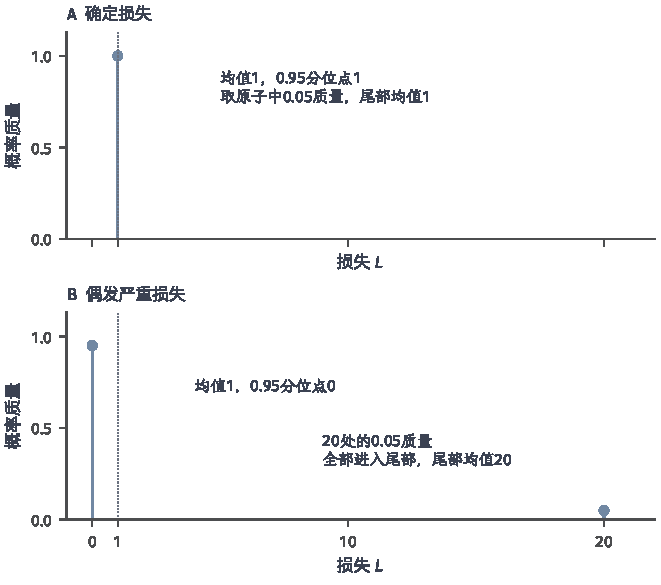
\includegraphics[width=112.000mm]{figures/10-reinforcement-learning/03-task-expansion-and-trustworthiness/matplotlib/rl-trustworthy-loss.pdf}
  \caption{两个教学损失分布，横轴为无量纲损失，纵轴为概率质量。粗实线和实心点表示原子，虚线标均值；图中文字说明用于计算CVaR的最差5\%质量，不是连续概率密度。}
  \label{fig:rl-trustworthy-loss}
\end{figure}

上面的定义假定损失分布已知。模型未知但允许运行当前策略时，可以直接用完整回合的样本估计累计损失，而不必先求转移核——因为我们只需要比较整个回合的后果，不需要知道每一步的转移核长什么样。设策略为$\pi_{\bm{\theta}}$，一回合损失为$L(\tau)$，把策略参数与尾部阈值组成联合目标
\[
  \Phi(\bm{\theta},\eta)
  =\eta+\frac{1}{1-\alpha}
      \mathbb E_{\tau\sim\pi_{\bm{\theta}}}(L(\tau)-\eta)_+.
\]
在环境不依赖策略参数、随机策略可微且支持不随参数突变，并能交换微分与期望的条件下，可用第~\ref{chap:rl-learning}~章的似然比方法求导。轨迹概率由逐步动作概率和环境转移概率相乘而成，环境项的参数导数为0，故其对数导数是
$\sum_{t=0}^{H-1}\nabla_{\bm{\theta}}\log\pi_{\bm{\theta}}(a_t\mid I_t)$。固定阈值，用超额损失加权这一轨迹得分，得到
\begin{equation}
  \nabla_{\bm{\theta}}\Phi
  =\frac{1}{1-\alpha}\mathbb E\left[
    (L-\eta)_+
    \sum_{t=0}^{H-1}\nabla_{\bm{\theta}}
       \log\pi_{\bm{\theta}}(a_t\mid I_t)\right].
  \label{eq:rl-trustworthy-tail-gradient}
\end{equation}
式~\eqref{eq:rl-trustworthy-tail-gradient}~中，未超过阈值的轨迹权重为0，超过阈值的轨迹按严重程度贡献策略更新。阈值本身的一个次梯度为
$1-(1-\alpha)^{-1}\mathbb P(L>\eta)$；在$L=\eta$处可以按$[0,1]$中的权重分配质量。算法~\ref{alg:rl-trustworthy-static-cvar}~据此同时更新阈值与策略，不需要把当前样本分位数当作真实分位数。

\begin{algorithm}[累计CVaR的轨迹更新]
  \label{alg:rl-trustworthy-static-cvar}
  \begin{algorithmic}[1]
    \Require 分位水平$\alpha$，时域$H$，批量$n$，步长序列，初值$\bm{\theta}^{(0)},\eta^{(0)}$
    \Ensure 候选策略及其阈值；可靠性另用留出评价样本验证
    \For{$k=0,\ldots,K-1$}
      \State 冻结当前参数，用$\pi_{\bm{\theta}^{(k)}}$独立启动$n$条轨迹，记录逐步损失并计算$L_j$
      \State 在旧参数、旧阈值上，用式~\eqref{eq:rl-trustworthy-tail-gradient}~的样本均值计算$\widehat{\bm{g}}_\theta$
      \State 计算$\widehat g_\eta=1-\frac{1}{n(1-\alpha)}\sum_j\mathbf 1\{L_j>\eta^{(k)}\}$，按需处理阈值处原子
      \State $\bm{\theta}^{(k+1)}=\bm{\theta}^{(k)}-\alpha_{\theta,k}\widehat{\bm{g}}_\theta$，
        $\eta^{(k+1)}=\eta^{(k)}-\zeta_k\widehat g_\eta$
    \EndFor
  \end{algorithmic}
\end{algorithm}

回到两条路线，可以直接检查梯度的行为含义。设出发时以概率$p=\operatorname{sigmoid}(\theta)$选偶发严重损失策略，否则选确定损失策略。对$0\leq p\leq1$，最差5\%质量由$0.05p$的损失20和$0.05(1-p)$的损失1组成，CVaR为$1+19p$。在$p=1/2$、最优阈值$\eta=1$处，精确策略梯度为$19p(1-p)=4.75$；沿负梯度更新会减小$\theta$，进而减少选择高尾部损失路线的概率。这个数由分布解析计算得到，不是训练实验的结果。

每批需要$nH$次交互与相应的策略求导，保存整批轨迹的空间也与$nH$成正比。经验分位数若通过排序求得，另需$O(n\log n)$；阈值次梯度只需$O(n)$。尾部估计还受有效回合数限制：用于最差部分的样本量约为$n(1-\alpha)$，这个数很小时，更新依赖极少数尾部回合，一整批也可能没有关键严重事件。误差还取决于损失尾部的大小及矩条件，不能只由这一回合数判断。

同批完整轨迹若既用于选择策略，又用于报告其尾部损失，还会引入选择偏差。模型轨迹能够减少真实交互，但模型在罕见区域的误差会直接影响尾部目标。百分位风险约束中的策略梯度和行动者--评论家方法同样需要估计风险、更新策略并调整约束，其局部收敛结论依赖特定假设；这些结论既不消除尾部估计误差，也不是任意神经网络训练的全局最优保证\scite{rl8-chow2018-percentile}

与无模型方法相对，已知有限时域模型时，也可以用动态规划求同一个静态目标，关键在于补齐状态。以累计损失
$L=\sum_{t=0}^{H-1}\gamma^t\ell_t$为例，只保存物理状态无法知道终点的超额损失，因而再记录已经积累的损失$z$。先固定出发前选定的$\eta$，把终端目标设为$(z-\eta)_+$，再用普通期望向后递推：
\begin{align}
  W_H^\eta(s,z)&=(z-\eta)_+, \nonumber\\
  W_t^\eta(s,z)&=\min_{a\in\mathsf A(s)}
       \mathbb E\!\left[
       W_{t+1}^\eta(s',z+\gamma^t\ell_t)\mid s,a\right].
  \label{eq:rl-trustworthy-augmented-risk}
\end{align}
再在出发前最小化
$\eta+(1-\alpha)^{-1}\mathbb E_{s_0\sim\mu_0}W_0^\eta(s_0,0)$。
每步把$\gamma^t\ell_t$加到累计量中，模型期望同时覆盖后继状态与本步损失；策略因此可以依赖时间、状态和已观察的累计损失。损失支持离散且有限时，可枚举可达$z$；$z$连续时，离散化或插值会扩大状态规模并引入误差。阈值仍属于事前承诺，途中重置为新的条件分位数会改变目标。另有增广方法保存尾部概率预算；原论文以尾部质量为参数，换成本章记号时应使用$1-\alpha$\scite{rl8-chow2015-cvar}

\begin{example}[静态CVaR的时间不一致]
  \label{ex:rl-trustworthy-time-inconsistency}
  设$H=2$且不折扣。$t=0$只有一个虚拟动作，损失为0，随后进入可观察的分支A或B，概率分别为0.1与0.9。$t=1$在B只有一个动作，损失固定为10；在A可以选safe，损失12，也可以选risky，损失以0.9概率为0、以0.1概率为20。决策者在$t=0$选择并承诺一个完整条件策略，在到达A后执行约定动作。

  取$\alpha=0.9$。承诺safe时，总损失分布为$10(0.9),12(0.1)$，CVaR为12。承诺risky时，分布为$0(0.09),10(0.9),20(0.01)$，最坏10\%由全部1\%的20和9\%的10组成，所以
  \[
    \operatorname{CVaR}_{0.9}(L_{\text{risky}})
       =\frac{0.01\times20+0.09\times10}{0.1}=11.
  \]
  事前准则严格选择risky。但一旦到达A，重新最小化条件CVaR，safe与risky的数值分别为12与20，因而严格选择safe。环境和可选动作没有改变，改变的是条件化之后用于定义尾部的概率质量。
\end{example}

反例中分支已被观察，冲突仍然发生：到达A后，定义最差10\%时不再计入B的概率质量。静态CVaR若只在原物理状态上套用普通Bellman递推，就可能丢掉事前评价的这层含义。式~\eqref{eq:rl-trustworthy-augmented-risk}~通过累计损失和固定阈值保留事前目标；若任务反而要求每个历史下都按当前条件重新评价，则需要下一小节的动态目标。

% Outline: 8.2.2
\subsection{逐阶段条件风险下的决策}
\label{sec:rl-trustworthy-dynamic-risk}

静态准则的时间不一致反例提示了另一种决策观：如果决策者不打算事先承诺，而是保留在每次取得新的观测、奖励或损失记录后重新决策的权利，就需要逐阶段地评价风险。到达A后，B已经被排除，未来方案可以只按A下的后果比较。\term{条件风险映射}（conditional risk mapping）执行的就是这一步：把下一阶段的不确定损失汇总成以当前已揭示记录为条件的风险数值。该数值在当前历史下已知，在更早时刻却仍可能随机。令$\mathcal F_t$为截至时刻$t$已揭示的状态或观测、已执行动作及已到达奖励或损失记录生成的$\sigma$代数；协议额外给出的公共信号也一并纳入。映射$\rho_t$把$\mathcal F_{t+1}$可测损失变成$\mathcal F_t$可测量。条件CVaR在式~\eqref{eq:rl-trustworthy-cvar}~中改用$\mathbb E[\cdot\mid\mathcal F_t]$，阈值也改为$\mathcal F_t$可测的随机变量；一般概率空间上使用本质下确界，即忽略零概率集合后仍成立的最大下界。有限树上，这等于在每个正概率历史的条件分布内分别优化阈值。不同策略的风险各自按其诱导分布计算；要比较这种排序能否跨时刻保持，则须在同一概率空间及同一组按时刻递增的$\sigma$代数下进行，不将不同策略的两条轨迹直接逐点配对。这样的几乎处处结论也不自动覆盖运行分布未支持的历史。

为将条件风险用于逐阶段交互控制，固定正整数时域$H$、$0\leq\gamma\leq1$、概率空间$(\Omega,\mathcal F,\mathbb P)$及递增$\sigma$代数族$\mathcal F_0\subseteq\cdots\subseteq\mathcal F_H$。令$L^\infty(\mathcal F_t)$表示相对于$\mathbb P$几乎处处有界、在$\mathcal F_t$下可测的随机变量。
  取归一化$\rho_t(0)=0$的一步条件风险映射$\rho_t:L^\infty(\mathcal F_{t+1})\to L^\infty(\mathcal F_t)$。对阶段损失$\ell_t\in L^\infty(\mathcal F_{t+1})$，定义
  \[
    \mathcal R_t
      =\rho_t(\ell_t+\gamma\mathcal R_{t+1}),
      \qquad \mathcal R_H=0.
  \]
  这一递归是\term{嵌套风险}（nested risk），即把后一步风险当作当前待评价的未来损失。
  动态风险族具有\term{时间一致性}（time consistency），如果对任意$0\leq u<v\leq H$和上述同一空间上的两个损失序列，它们在$u,\ldots,v-1$几乎处处相同，且$v$时刻的条件风险几乎处处满足$\mathcal R_v\leq\widetilde{\mathcal R}_v$，就有
  $\mathcal R_u\leq\widetilde{\mathcal R}_u$。
  所有几乎处处比较均相对于同一个$\mathbb P$。有界空间使逐层输入和输出仍在映射定义域内；无界损失的动态风险须另给可积性与定义域封闭条件，不能只沿用静态CVaR的可积假设。

共同概率空间可以先按一棵固定的随机树理解：分支、分支概率和前段损失不变，只比较两套后续损失。例如两个叶节点上的损失分别为$X=(2,4)$与$Y=(3,5)$，就能在同一叶节点逐项比较$X\leq Y$；单调的条件风险把这种排序逐层向前传递。这里检查的是同一条件风险规则怎样评价不同损失，并不是把两个机器人各自运行得到的轨迹强行配对。

控制优化还要加入动作对后继分布的影响。不同动作可以产生不同的下一状态分布，因而下面分别用$\rho_{t,s,a}$表示给定状态动作后的一步条件风险。先按每个动作对应的条件分布计算风险，再比较动作，与前面的共同空间排序性质并不冲突。

时间一致性保留跨时刻的排序：两方案前段损失相同，若以后在每个可能历史下一个方案的条件风险都不更高，较早评价也不应把它排得更差。各$\rho_t$单调时，将$v$时刻的不等式逐层代入递归，就能传到$u$。这一论证控制的是条件风险排序，并未断言每条轨迹都没有损失。动态风险及其Markov表示的系统论述见原始工作\scite{rl8-ruszczynski2010-risk}

在示例~\ref{ex:rl-trustworthy-time-inconsistency}~中，每层采用$\alpha=0.9$的条件CVaR。先在A内汇总叶节点，risky得到20，safe得到12；B的风险为10。再汇总分支风险$20(0.1),10(0.9)$，risky的嵌套风险为20，safe则为12。图~\ref{fig:rl-trustworthy-risk-tree}~对照这两种运算：静态准则直接使用叶节点的联合概率，嵌套准则先把分支后果压成条件风险。选择从risky变为safe，来自评价对象改变，而非静态求解精度提高。

\begin{figure*}[t]
  \centering
  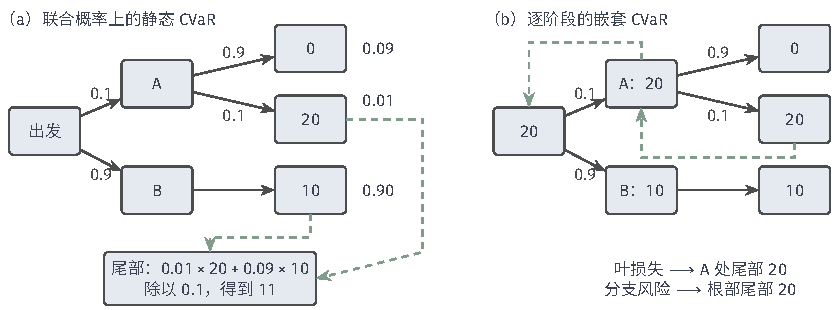
\includegraphics[width=141.390mm]{figures/10-reinforcement-learning/03-task-expansion-and-trustworthiness/tikz/rl-trustworthy-risk-tree.pdf}
  \caption{同一教学决策树的两种风险汇总，均取$\alpha=0.9$、$H=2$且不折扣。图中展示承诺risky的分支；实线表示随机转移，带文字的回传箭头表示风险计算。safe只需将A的两个叶节点替换为固定损失12。}
  \label{fig:rl-trustworthy-risk-tree}
\end{figure*}

分支树可以逐层回传，状态价值递推却还要求状态保存决定后继条件分布和风险映射的历史记录、累计损失或剩余预算。这里要求给定$(t,s,a)$后，后继条件分布、风险映射及其水平不再依赖未记录的历史；各映射在相应条件分布的有界后继变量上定义，并满足单调性，使后续风险的改善能够传到当前评价。设动作确定后，一步损失$\ell(s,a)$已知，$\rho_{s,a}$只评价后继状态上的随机量。若风险满足平移等变性，即加上当前已知常数会使风险增加同一常数，就能把这一步损失移到映射外。有限时域Markov风险问题于是可向后归纳为
\begin{equation}
  V_t(s)=\min_{a\in\mathsf A(s)}
    \{\ell_t(s,a)+\rho_{t,s,a}(\gamma V_{t+1}(s'))\},
  \qquad V_H=0.
  \label{eq:rl-trustworthy-risk-bellman}
\end{equation}
式~\eqref{eq:rl-trustworthy-risk-bellman}~先评价每个动作下的未来风险，再选损失风险最小的动作。一步损失若也随机，须将$\ell_t+\gamma V_{t+1}$一起放入联合分布的风险映射；风险水平若依赖剩余预算或历史，相应的剩余预算或历史记录也须进入状态。这里采用确定性Markov动作选择。允许随机动作时，还要规定风险在随机化之前还是之后评价，否则算子所优化的目标并未确定。

\begin{theorem}[折扣风险算子的压缩性]
  \label{thm:rl-trustworthy-risk-contraction}
  设状态集$S$及每个可行动作集$\mathsf A(s)$有限且非空，确定阶段损失$\ell(s,a)$有界，$0<\gamma<1$。对每个$(s,a)$，固定后继条件分布及风险规则，映射$\rho_{s,a}:\mathbb R^{|S|}\to\mathbb R$在所有有限后继值向量上有定义，迭代中不改变；所需历史已计入状态。
  每个映射满足单调性，即逐后继状态$X\leq Y$推出$\rho_{s,a}(X)\leq\rho_{s,a}(Y)$，并对任意实常数$b$满足平移等变性
  $\rho_{s,a}(X+b)=\rho_{s,a}(X)+b$。
  对已经按声明的风险问题建立的算子
  \[
    (\mathcal B V)(s)=\min_{a\in\mathsf A(s)}\{\ell(s,a)+\rho_{s,a}(\gamma V(s'))\},
  \]
  对任意$V,W\in\mathbb R^{|S|}$，有$\lVert\mathcal B V-\mathcal B W\rVert_\infty\leq\gamma\lVert V-W\rVert_\infty$。
  因而该算子有唯一不动点，反复应用$\mathcal B$从任意有限初值收敛到该点。
\end{theorem}
\begin{proof}
  令$\varepsilon=\lVert V-W\rVert_\infty$。对所有后继状态，
  $\gamma W-\gamma\varepsilon\leq\gamma V\leq\gamma W+\gamma\varepsilon$。
  单调性把不等式传入$\rho_{s,a}$，平移等变性把两端的常数移出，得到
  \[
    \rho_{s,a}(\gamma W)-\gamma\varepsilon
      \leq\rho_{s,a}(\gamma V)
      \leq\rho_{s,a}(\gamma W)+\gamma\varepsilon.
  \]
  记每个动作的花括号表达式为$q_V(s,a)$和$q_W(s,a)$，则
  $|q_V-q_W|\leq\gamma\varepsilon$。对所有动作的下界取最小值，得
  $(\mathcal B V)(s)\geq(\mathcal B W)(s)-\gamma\varepsilon$；取上界的最小值，得反向界。因此所需无穷范数界成立。

  $\mathbb R^{|S|}$配无穷范数是非空完备度量空间，上述算子把它映回自身，且压缩因子为$\gamma<1$。压缩不动点结论因此给出唯一不动点及任意有限初值的几何收敛，并有
  $\lVert V^{(k)}-V^\star\rVert_\infty\leq\gamma^k\lVert V^{(0)}-V^\star\rVert_\infty$。
  相关基础可参考\BookChapterRef{chap:metric-spaces}{卷1《数学准备：计算、分析与几何》“度量空间”章}。这里保证的是已经按声明风险建立的固定算子的求解，不保证环境或风险模型本身正确。
\end{proof}

证明用单调性传递上下界，用平移等变性移出误差常数，没有使用正齐次性，因而将折扣留在$\rho(\gamma V)$内部即可。它回答的是价值迭代是否收敛。不动点是否代表希望求解的风险目标，还须核对时间一致性、状态所保存的历史与预算和允许策略类，数值压缩性本身不证明这些建模条件。

以已知有限模型的条件CVaR价值迭代为例，每轮先冻结$V^{(k)}$。对每个$(s,a)$，列出后继值$\gamma V^{(k)}(s')$及概率，按值排序并从最大值累计$1-\alpha$质量，再由式~\eqref{eq:rl-trustworthy-tail-mass}~求风险；加上$\ell(s,a)$后，对动作取最小值。排序是在寻找严重损失尾部，动作最小化则是在改善决策。迭代到残差
$\lVert\mathcal B V^{(k)}-V^{(k)}\rVert_\infty\leq(1-\gamma)\epsilon$时，
压缩界与三角不等式给出
$\lVert V^{(k)}-V^\star\rVert_\infty\leq\epsilon$。
在两阶段树上，从终端0开始，A的回传立即得到$\min(12,20)=12$，B得到10，根部再得到12，完成一次可复核的向后计算。

记状态数为$m$、每状态最多$b$个动作，稠密转移下每轮排序更新需$O(bm^2\log m)$，模型存储需$O(bm^2)$。若只有指定状态动作的采样接口，就需用独立后继批次估计条件分布；条件CVaR是分布的非线性函数，单个后继样本的风险一般不能无偏估计总体风险。每步近似算子误差若一致不超过$e$，迭代误差满足
$\Delta_{k+1}\leq\gamma\Delta_k+e$，长期误差上限为$e/(1-\gamma)$。
因此，风险策略梯度需要与嵌套目标相符的风险权重，分布评论家则需估计相应的条件后果分布。把期望评论家的价值预测换成尾部分位数，只改变了一个预测量；还须推导它如何参与目标和更新，才能得到所声明的风险算法。

% Outline: 8.3
\section{不确定环境下的鲁棒决策}
\label{sec:rl-trustworthy-robust}

风险准则处理的是一个固定概率模型内部的随机性。现在放宽“模型已知且准确”这个前提：部署环境可能与训练时不同，问题转为同一策略能否在允许的变化范围内维持要求。注意这里不假设各环境以某个概率出现——工程师通常只知道摩擦的物理区间、传感器的误差规格，而不知道“今天是干地还是湿地”的概率，因此不能简单取期望，只能保证整个范围内的最坏表现。变化进入系统的位置不同，应对手段也不同。图~\ref{fig:rl-trustworthy-channels}~固定交互闭环，区分三个扰动位置：摩擦变化影响真实状态转移，传感读数修改影响策略读取的观测，制动力削弱影响请求动作的实际执行。对抗训练是在这些位置搜索不利变化的求解手段，不是第四种扰动对象。

\begin{figure*}[t]
  \centering
  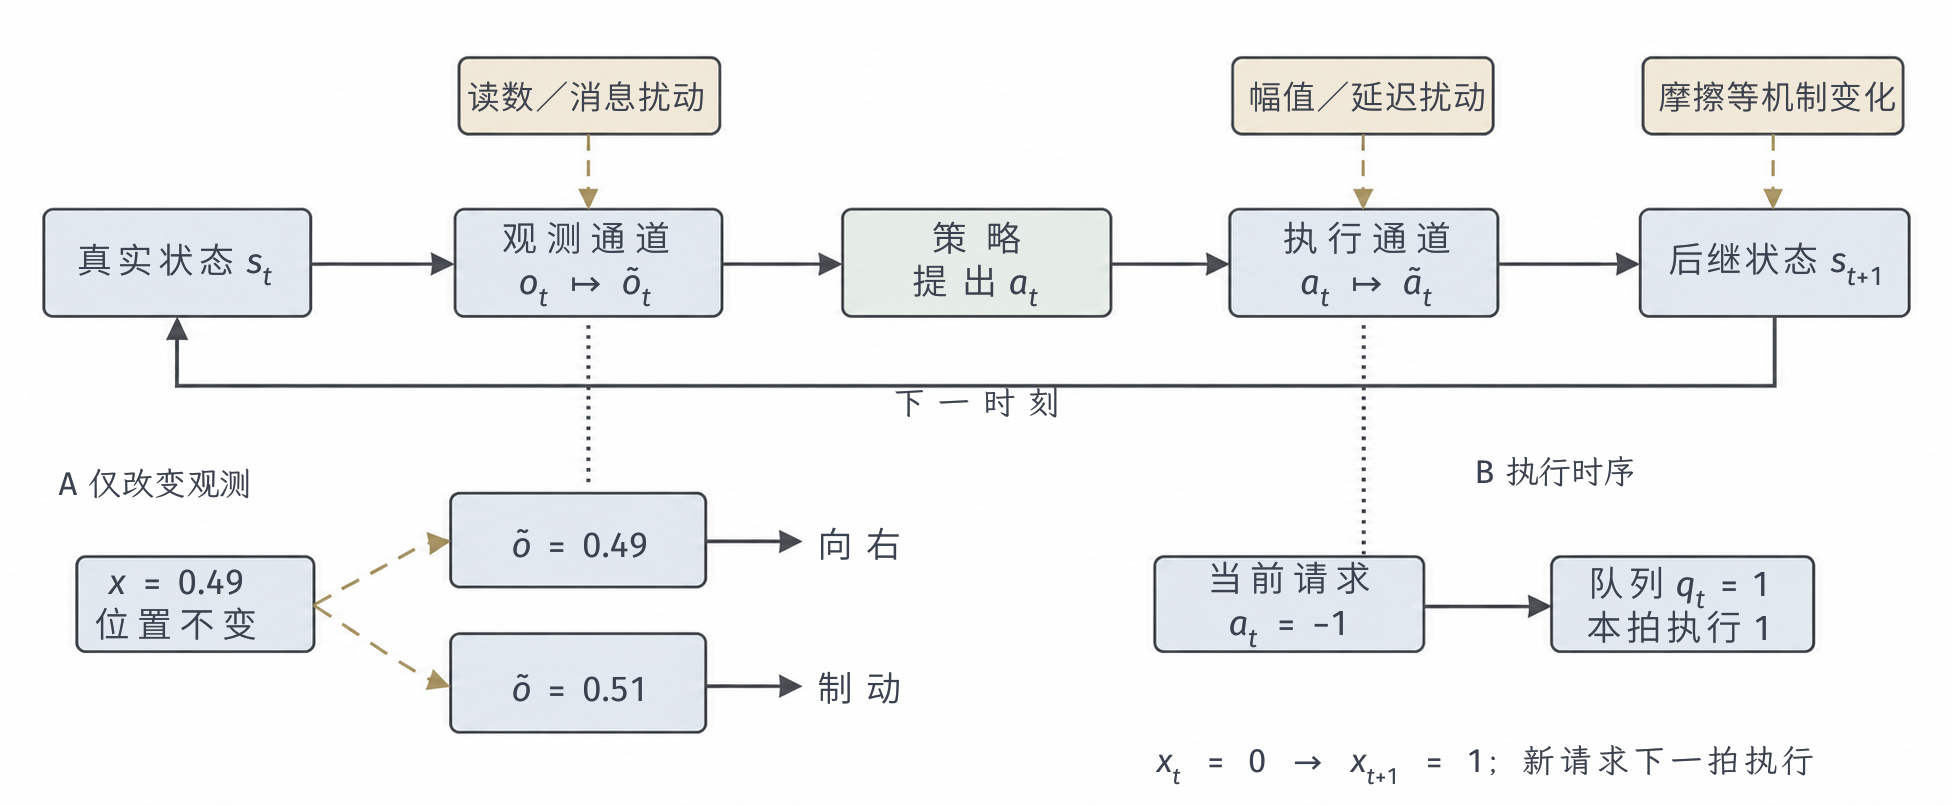
\includegraphics[width=157.400mm]{figures/10-reinforcement-learning/03-task-expansion-and-trustworthiness/generated/rl-trustworthy-channels/figure.png}
  \caption{扰动进入交互闭环的三个位置。实线传递状态、观测与动作，虚线表示不同扰动权限。下方两个局部面板分别只突出观测误差和执行延迟，二者均不等于直接改变当前真实位置。点状引线只定位下方对应通道的局部示意，不表示额外运行路径。}
  \label{fig:rl-trustworthy-channels}
\end{figure*}

% Outline: 8.3.1
\subsection{环境机制变化下的鲁棒决策}
\label{sec:rl-trustworthy-mechanism}

先处理动力学本身的不确定性。摩擦系数的点估计0.6给出标称模型$\widehat T$，用它规划相当于赌真实摩擦恰好是0.6；物理测量若只支持区间$[0.4,0.8]$，则给出一族可能转移核$\mathcal U$，鲁棒规划要在这一族上都站得住。前者适合预测标称表现，后者适合检查整个允许范围内的不利表现。固定奖励$R$和初态分布$\mu_0$，只让转移核变化，从而单独识别动力学不确定性的影响。区间没有规定各模型出现的概率，因而尚不能对模型作概率平均；即使另给概率权重，平均回报较高也可能掩盖某个允许模型下的低回报。要为集合内每个模型提供统一下界，就先对同一策略取回报的下确界，再选择这个下界最大的策略；每个模型内部的随机轨迹仍由$J_T(\pi)$取期望。

\begin{definition}[最坏情形回报]
  \label{def:rl-trustworthy-robust-return}
  固定有限状态动作、非空可行动作、有界奖励$R$、初态分布$\mu_0$和$0\leq\gamma<1$。令$\mathcal U$为非空允许转移核集合，各核均给出每个状态动作下的概率分布；$J_T(\pi)$是在核$T$下由$\mu_0$启动、按策略$\pi$运行的期望折扣回报。给定非空合法候选策略类$\Pi$，其中每条策略均按其获准历史选择合法动作。对固定$\pi\in\Pi$，鲁棒回报及该类中的最优值为
  \[
    J_{\mathrm{rob}}(\pi)=\inf_{T\in\mathcal U}J_T(\pi),
    \qquad J_{\mathrm{rob}}^\star=\sup_{\pi\in\Pi}J_{\mathrm{rob}}(\pi).
  \]
  集合$\mathcal U$描述允许的环境，而不是轨迹中随机转移结果的集合。若奖励或初态也不确定，应把它们与$T$一起列入模型集合。
  候选类$\Pi$还须指定允许确定性、随机化和历史依赖的范围。最优值能否由某条策略取到需另证；保证取到以后，才可把上确界写成最大值。
\end{definition}

区间可以来自设备的物理界，也可以来自转移记录的联合置信区域；两种来源的保证不同。若$\mathcal U=\mathcal U(D)$由转移记录$D$构造，模型假设还需附带统计覆盖事件
$\{T_{\text{真}}\in\mathcal U(D)\}$。在该事件上，任何被评价策略都有
$J_{T_{\text{真}}}(\pi)\geq\inf_{T\in\mathcal U}J_T(\pi)$。
这是集合内的确定性比较：真实模型只要被包含，最坏回报便是其回报下界。集合若以至少$1-\delta$的概率覆盖真实模型，才能进一步形成带置信水平的声明。集合过小可能漏掉真实环境，过大则可能降低可保证的回报，付出不必要的保守代价。鲁棒MDP需要同时说明集合结构和转移记录所给出的置信区域\scite{rl8-wiesemann2013-robust}

最坏回报定义是对整个模型一次性取最坏，但Bellman备份每次只处理一个状态动作；要让局部选择拼出一个合法的全局最坏环境，集合还须能够分解。\term{状态--动作矩形性}（state-action rectangularity）指
$\mathcal U=\prod_{s,a}\mathcal U_{s,a}$，也就是从各局部集合任选一个转移分布，组合后仍是允许模型。相应动态对手看到当前状态和已选动作后，在$\mathcal U_{s,a}$中选择下一步分布，不受跨状态或跨时间的共享剩余预算约束。下面采用最小值写法时，还要求各$\mathcal U_{s,a}$是概率单纯形中的非空紧集，使连续的线性目标能够取到最小值；若只知道局部集合非空而不能保证取到，则应把内层写成下确界。按这些条件与权限得到
\begin{equation}
  (\mathcal B_{\mathrm{rob}}V)(s)
    =\max_{a\in\mathsf A(s)}
      \left\{R(s,a)+\gamma
        \min_{p\in\mathcal U_{s,a}}\sum_{s'}p(s')V(s')\right\}.
  \label{eq:rl-trustworthy-robust-bellman}
\end{equation}
式~\eqref{eq:rl-trustworthy-robust-bellman}~的外层最大化回报，内层最小化给定动作下的后继价值。先选动作再让对手选择分布，正是前述对手读取当前状态与动作的权限；若对手须在看到动作前承诺一个跨动作共享的参数，允许的局部选择会变少，不能直接沿用同一算子。

\begin{theorem}[矩形鲁棒Bellman算子的压缩性]
  \label{thm:rl-trustworthy-robust-contraction}
  设状态集$S$及可行动作集$\mathsf A(s)$有限且非空，奖励$R(s,a)$有界，$0<\gamma<1$，每个$\mathcal U_{s,a}$都是$S$上概率单纯形中的非空紧集。令全局转移核集合为$\mathcal U=\prod_{s,a}\mathcal U_{s,a}$，对手在当前状态和动作已知后选择本步分布，不受跨步共享约束；状态是双方所用历史的共同充分表示。固定这些奖励、集合与权限后，式~\eqref{eq:rl-trustworthy-robust-bellman}~作为$\mathbb R^{|S|}$上的算子，在无穷范数下是$\gamma$压缩映射。
\end{theorem}
\begin{proof}
  令$\varepsilon=\lVert V-W\rVert_\infty$。对任意概率向量$p$，
  \[
    \left|\sum_{s'}p(s')V(s')-\sum_{s'}p(s')W(s')\right|
      \leq\sum_{s'}p(s')\varepsilon=\varepsilon.
  \]
  记内层最小值为$m_V,m_W$。上式对集合中每个$p$都成立，故
  $\sum pV\geq\sum pW-\varepsilon\geq m_W-\varepsilon$，取最小值得
  $m_V\geq m_W-\varepsilon$。由于紧性保证$W$的最小点$p_W$存在，
  $m_V\leq\sum p_WV\leq m_W+\varepsilon$。于是$|m_V-m_W|\leq\varepsilon$。
  加入相同的$R(s,a)$并乘以$\gamma$，每个动作的表达式相差至多$\gamma\varepsilon$。
  对各动作的上下界分别取最大值，得到
  \[
    (\mathcal B_{\mathrm{rob}}W)(s)-\gamma\varepsilon
      \leq(\mathcal B_{\mathrm{rob}}V)(s)
      \leq(\mathcal B_{\mathrm{rob}}W)(s)+\gamma\varepsilon.
  \]
  对状态取最大绝对差，结论成立。不动点存在、唯一及价值迭代收敛，由定理~\ref{thm:rl-trustworthy-risk-contraction}~中使用的非空完备空间上的压缩不动点结论得到。
\end{proof}

压缩证明控制的是数值迭代，矩形性则把局部最坏选择接成合法的全局环境。不动点处，各状态可取一个外层最优动作，各状态动作可取一个内层最差分布；由于这些分布可自由组合，它们共同给出$T^\star\in\mathcal U$。固定平稳Markov策略时，将外层最大化换成按$\pi(a\mid s)$平均，保留各动作下的内层最小化，就得到该策略在矩形模型族中的最坏回报评价。

历史依赖策略还需在状态中保留所用记忆，但状态增广不自动产生矩形性。若以$(s,m)$表示物理状态与记忆，同一个物理参数在不同记忆副本间共享的关系仍须保留；不能仅因$m$不同，就允许对手分别选择彼此不相容的参数。否则得到的是更大的不确定集合，后面的共享参数示例~\ref{ex:rl-trustworthy-coupling}~说明了这种扩大怎样改变最坏回报。局部备份与动态对手的对应，由有限时域逐步归纳和无限时域折扣极限建立；有限时域模型族还须允许各时刻局部分布独立组合。空间上的矩形性并不自动赋予时间上的自由变化，任意耦合集合也不满足这套分解条件。

求解式~\eqref{eq:rl-trustworthy-robust-bellman}~时，置信多面体使内层成为线性目标$\sum pV$的线性规划；只有两个后继状态的概率区间时，线性目标在端点取最小值。教学例取后继价值10与0、$\gamma=0.9$、当前奖励0，好状态概率$p\in[0.7,0.9]$。最坏选择为$p=0.7$，备份为$0.9\times0.7\times10=6.3$；标称$p=0.8$时为7.2。另一动作若确定到达价值7.5的后继，其备份为6.75，于是标称选择第一个动作，鲁棒选择第二个动作。

每轮冻结旧价值，逐状态动作求内层最小值，再取外层最大值。记一次内层优化代价为$C_{\text{内}}$，每轮需$O(mbC_{\text{内}})$。内层求解残差、模型集合估计误差和价值逼近误差影响不同步骤，应分别记录，不能只报告最终迭代残差。

\begin{example}[共享参数不能随状态独立取坏值]
  \label{ex:rl-trustworthy-coupling}
  一个两阶段教学任务以相同概率从$s_1,s_2$启动，各只有一个动作，第一步奖励0。下一步到达成功状态得到奖励1，失败状态得到0，随后终止。整个环境共享一个固定未知参数$\vartheta\in[0,1]$，成功概率分别是
  $p_1=\vartheta$与$p_2=1-\vartheta$。
  对任意合法环境，初态平均回报都为
  $\gamma(p_1+p_2)/2=\gamma/2$。
  如果只保留每个概率各自属于$[0,1]$，逐状态最坏选择会取$p_1=p_2=0$，得到回报0；然而不存在同时产生这两个概率的$\vartheta$。
\end{example}

图~\ref{fig:rl-trustworthy-rectangular}~的斜线给出共享参数真正允许的组合，方形则允许局部概率各自取坏值。扩大集合的算子即使严格收敛，也是在解更保守的另一个问题。共享参数若能由历史观测逐渐识别，新观测还可能通过辨识共享参数来改善后续控制；保留参数信念或相关历史才能利用它，将每次访问都当作对手重新任意选参数会丢掉这一机会。

\begin{figure}[htbp]
  \centering
  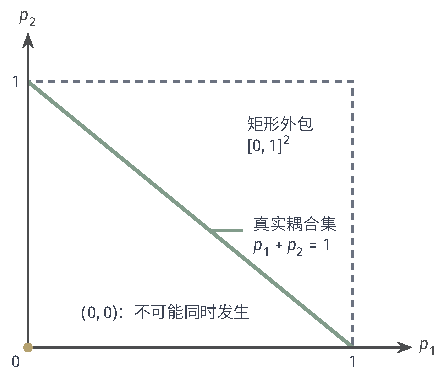
\includegraphics[width=75.805mm]{figures/10-reinforcement-learning/03-task-expansion-and-trustworthiness/tikz/rl-trustworthy-rectangular.pdf}
  \caption{教学耦合集$\{(p_1,p_2):p_1+p_2=1\}$与矩形外包$[0,1]^2$。方形左下角给出局部最坏选择，却不属于共享参数模型。坐标是两状态的成功概率。}
  \label{fig:rl-trustworthy-rectangular}
\end{figure}

“分布鲁棒”仍须说明哪个分布不确定。可能变化的是后继状态转移分布$p(\cdot\mid s,a)$，也可能是随机环境参数$\vartheta$的分布$\nu$；后一种问题优化
$\inf_{\nu\in\mathfrak U}\mathbb E_{\vartheta\sim\nu}J_{T_\vartheta}(\pi)$。
回合开始时抽取模型并保持不变，会使整段轨迹共享参数；每步重新抽取通常产生不同过程。Xu与Mannor的分布鲁棒MDP用参数分布的嵌套集合约束表示已知的参数概率或概率界，并建立相应状态分解与求解条件；这些条件不是把任意参数分布歧义集逐状态拆开的许可\scite{rl8-xu2010-distributional}

表~\ref{tab:rl-trustworthy-uncertainty}~按不确定对象对齐集合来源和求解条件。其他参与者造成的转移变化，还须符合第~\ref{chap:rl-multi-agent}~章的联合行为模型，不能擅自赋予其任意局部变化权限；识别未知参数后再适应，则涉及第~\ref{chap:rl-transfer}~章的任务推断。

\begin{table}[htbp]
  \centering
  \begin{tabularx}{\linewidth}{@{}>{\raggedright\arraybackslash}p{20mm}XX@{}}
    \toprule
    不确定对象 & 集合来源与矩形条件 & 内层求解及保证范围 \\
    \midrule
    参数$\vartheta\in\Theta$ & 物理区间或联合置信集；共享参数通常耦合状态 & 在$\Theta$上优化；覆盖整个参数族，不自动支持局部备份 \\
    转移分布$p\in\mathcal U_{s,a}$ & 距离球、矩或似然约束；须说明各对之间能否自由组合 & 线性、凸或专门分布优化；只覆盖声明集合 \\
    参数分布$\nu\in\mathfrak U$ & 对模型参数随机性的矩、支持或概率质量约束 & 对分布求最坏期望；需说明参数抽取时机及依赖 \\
    \bottomrule
  \end{tabularx}
  \caption{三种不同层次的不确定性。置信覆盖是构造集合的额外统计性质，不由“鲁棒”或“分布鲁棒”的名称保证。}
  \label{tab:rl-trustworthy-uncertainty}
\end{table}

% Outline: 8.3.2
\subsection{观测信息受扰下的鲁棒决策}
\label{sec:rl-trustworthy-observation}

第二类扰动不改动物理世界，而在机器人感知世界的读数上做手脚——这对应传感器误差或针对感知的攻击。摩擦模型的不确定性已经明确，下面固定真实动力学与路线，只改变传感器报告。记真实状态为$s_t$，原始观测为$o_t$，受扰观测为$\widetilde o_t$，策略能够使用的历史为
$\widetilde I_t=(\widetilde o_0,a_0,\ldots,\widetilde o_t)$。
为确定最坏情形，先声明威胁模型，也就是扰动者的修改范围与观测、策略参数和历史读取权限。例如传感器误差规格给出$\epsilon$，扰动者在原始观测产生后、策略采样动作前选择
$\widetilde o_t\in\mathcal B_\epsilon(o_t)=\{o:\lVert o-o_t\rVert_\infty\leq\epsilon\}$；
它能看到当前原始观测和策略参数，不能看到未来噪声或尚未采样的动作。总预算若还满足$\sum_t\lVert\widetilde o_t-o_t\rVert\leq B$，先前修改会消耗后续权限，剩余预算便须进入对手状态。逐步误差界与整回合预算约束不同，两者产生的最坏情形也不同。

图~\ref{fig:rl-trustworthy-channels}~的观测面板固定真实位置$x=0.49$。教学策略在读数小于0.5时向右，否则制动；读数0.49与0.51都满足$|\widetilde o-x|\leq0.02$，却触发不同动作。机器人没有因此移动到0.51，变化只发生在策略读取的观测。若测试只覆盖$\widetilde o=0.48,0.49$，就没有触及允许集合另一侧的动作切换；两个测试通过不足以覆盖整个误差范围。

训练时，可以先冻结当前策略，在允许预算内搜索使回报降低的观测序列，再用受扰轨迹更新策略，最后以未参与更新的扰动规则和启动条件检验。令$\iota_t$表示威胁模型允许扰动者在时刻$t$读取的观测、策略参数与历史记录；在上述示例中，它只能由当前原始观测、策略参数以及协议明确允许的记录组成。以无记忆确定性连续动作策略为例，若有只依赖$\iota_t$与动作的可微一步价值代理，可从$o_t$初始化并进行投影梯度搜索：
\[
  \widetilde o^{(j+1)}
   =\operatorname{Proj}_{\mathcal B_\epsilon(o_t)}
      \left(\widetilde o^{(j)}
       -\xi\nabla_{\widetilde o}
          \widehat Q(\iota_t,\pi_{\bm{\theta}}(\widetilde o^{(j)}))\right).
\]
这里$\xi>0$是搜索步长，$\widehat Q$按奖励回报计分。负梯度搜索以降低这一代理价值为目标，投影使修改后的观测仍在允许误差集合内；步长与代理光滑性不合适时，单步也未必降低目标。该式只处理逐步误差球，若另有整回合预算，还须限制本步支出并更新剩余预算。模拟训练若额外把真实状态$s_t$输入评论家，就属于特权训练：只有$s_t$能由$\iota_t$确定，或最终扰动规则已经去除特权输入并能仅凭$\iota_t$执行时，该规则才属于上述威胁模型的允许集合；否则它评价的是允许读取额外真实状态或历史的另一威胁模型，不能充当前允许规则的攻击证据。无论依据哪些允许读取的观测或记录，投影搜索都只是在局部代理上寻找不利观测，没有保证整条轨迹最坏。随机策略须对动作分布下的期望价值求导，不能把分布本身当作动作输入$\widehat Q$；有记忆策略则须把协议允许的受扰历史纳入$\iota_t$，并保留它对策略内部状态的影响。

生成受扰样本后，可用第~\ref{chap:rl-learning}~章的策略更新提高受扰回报。更新后的参数又改变下一轮攻击目标，因此对手梯度与策略梯度须分开计算。每步若搜索$K_{\text{攻}}$次，梯度计算代价约增为普通采样的该倍数；增加搜索量也不等于证明搜索完备。

除了受扰训练，还可以减少观测所对应的状态歧义。鲁棒状态估计将读数转成与误差模型相容的状态集合，历史方法借助动力学和多次观测排除部分状态，观测保护则修复或拒绝可疑读数。它们分别依赖有效误差界、足够准确的动力学或可识别的异常观测。

修复器输出$\widehat o$若仍有误差$\|\widehat o-o\|\leq e$，要将它传到行为上，还需确定性连续动作策略在该区域满足Lipschitz条件，即观测距离能按固定比例控制动作距离。此时
$\|\pi(\widehat o)-\pi(o)\|\leq L_\pi e$；进一步得到回报或安全界，还需价值或闭环动力学的敏感性界。前述阈值策略在切换面附近不满足这种连续性估计。信念与历史状态的构造见第~\ref{chap:rl-information}~章。

把满足前述修改范围、可读观测与记录及预算的整回合扰动规则组成集合$\mathcal N$，以$\nu$表示其中一条规则；此处$\nu$不是上一小节的参数分布。固定策略与规则后，$J(\pi,\nu)$是在其诱导轨迹分布下的期望回报，定义真实最坏回报$J_{\min}=\inf_{\nu\in\mathcal N}J(\pi,\nu)$。近似搜索若找到允许规则$\widehat\nu\in\mathcal N$，则
$J_{\min}\leq J(\pi,\widehat\nu)$：该规则的期望回报对最坏回报只是一个上界，单次攻击样本或有限样本均值却不必满足这一确定性比较。只有另外证明内层误差
$J(\pi,\widehat\nu)-J_{\min}\leq e_{\text{攻}}$，才能得到
$J_{\min}\geq J(\pi,\widehat\nu)-e_{\text{攻}}$。
若期望回报也由样本估计，所得下界还须扣除相应统计误差。近似攻击只找到允许集合中的一个候选，其他扰动可能更坏。覆盖全部允许的观测扰动规则，仍需搜索完备性、可验证的内层误差界或形式化分析；若干攻击下表现良好只支持已测条件下的结论。

% Outline: 8.3.3
\subsection{动作执行受扰下的鲁棒决策}
\label{sec:rl-trustworthy-actuation}

第三个扰动位置在感知之后、物理世界之前：执行机构。前两小节默认“策略决定的动作会被精确执行”，但真实的电机和刹车都有幅值误差、饱和与延迟。即使观测准确，策略请求制动也不意味着制动力立即足量施加。记请求动作为$a_t$，实际动作为$\widetilde a_t$。幅值误差可写成$\widetilde a_t=a_t+e_t$、$\|e_t\|\leq\epsilon_a$，其中$\epsilon_a$来自执行器误差规格；若有饱和，还须把实际动作限制在设备能力内。动作篡改须声明攻击者何时读取请求，延迟须声明队列和最大滞后。图~\ref{fig:rl-trustworthy-channels}~的执行面板区分了请求与实际动作。

固定一拍延迟时，下一步执行的是旧请求，物理系统满足
$x_{t+1}=f(x_t,a_{t-1},w_t)$。当前状态$x_t$和请求$a_t$不足以确定下一步分布，还须知道队列内容。把它记为$q_t=a_{t-1}$并增广状态
$z_t=(x_t,q_t)$，得到
\begin{equation}
  x_{t+1}=f(x_t,q_t,w_t),\qquad q_{t+1}=a_t.
  \label{eq:rl-trustworthy-delay}
\end{equation}
若$w_t$在给定$z_t,a_t$后由固定核抽取，增广状态就恢复了马尔可夫转移。教学系统$x_{t+1}=x_t+\widetilde a_t$在$x_t=0,q_t=1$时，即使请求$a_t=-1$，下一步仍到$x_{t+1}=1$；新请求只将队列改为$-1$。省略队列会遗漏真正决定本步运动的动作，进而误判制动请求的效果。

执行误差集合已知时，应对每个请求动作评价其可能的实际效果。以回报价值$V$为例，集合只规定允许的执行误差，没有给这些误差的概率权重；要覆盖集合中每种误差，就取后继期望价值的下确界，而不能用若干误差的平均值代替。内层最坏后继价值为
\begin{equation}
  \inf_{e\in E(s,a)}
       \mathbb E\!\left[V\bigl(f(s,a+e,w)\bigr)\right].
  \label{eq:rl-trustworthy-actuation-backup}
\end{equation}
这里$E(s,a)$来自设备误差界或所声明的攻击权限，$e$由扰动者选择；$w$是按声明条件分布抽取的其他随机扰动。$f$将实际动作$a+e$映射到后继状态，$V$衡量其未来收益。先选择$e$再对$w$求期望，表示对手不能预见尚未抽取的$w$。完整备份还须加入即时奖励与折扣，并按实际对手权限组织外层动作优化；即时奖励若也依赖$e$，须纳入同一个内层优化。

可用模型或真实交互搜索不利执行动作，再训练策略提高受扰回报；近似搜索的证据方向仍与上一小节相同。反馈补偿则从实际运动估计误差，修正下一次请求。这需要足够快的测量、可辨识的误差和剩余控制能力；完全失去制动力或超过响应能力的延迟，不会因加入反馈而变得可补偿。

若执行通道在给定当前状态动作后与更早历史条件独立，且条件分布$K$固定，可以将它积分进有效转移核
\[
  T_{\mathrm{eff}}(s'\mid s,a)
    =\int T(s'\mid s,\widetilde a)\,K(d\widetilde a\mid s,a).
\]
这个积分把固定、无记忆的执行通道吸收到转移模型中。有记忆的延迟、相关误差或对手剩余预算不能这样无损消去；实际动作不可见时，还可能需要由历史推断队列或误差状态。保存一拍离散动作队列会使表格规划状态数从$m$增至$m|\mathsf A|$，多拍队列又可使规模指数增长。

模型学习也须区分请求与执行：学习物理模型$T(s'\mid s,\widetilde a)$需要实际动作，学习包含执行通道的$T_{\mathrm{eff}}(s'\mid s,a)$则需要请求动作和固定通道协议。日志因而应同时保存两种动作及干预原因，避免把通道变化归给物理动力学。补偿即使提高平均回报，也未必排除危险动作；实际动作是否满足安全要求，还须用下一节的约束与保护条件判断。

% Outline: 8.4
\section{安全约束下的策略学习与保护}
\label{sec:rl-trustworthy-safety}

鲁棒回答的是“环境变了策略还灵不灵”，但即使环境范围固定，仍有一个更直接的问题没有回答：哪些行为本身就不被允许？这正是第三类要求。导航中，平均危险区停留时间不超过预算、整回合碰撞概率不超过阈值、任何时刻都不越界，是三种不同要求：前两种允许个别轨迹违约（只要总体的平均值或概率达标），最后一种在声明范围内不允许违约——哪怕只发生一次也不行。它们无法互相替代：平均停留时间短不代表不会碰撞，碰撞概率低也不代表绝对不会越界。表~\ref{tab:rl-trustworthy-constraint-types}~按判定方式加以区分。交互记录的来源、动力学知识和保护器权限决定求解手段，但不会把一种约束变成另一种。

\begin{table}[htbp]
  \centering
  \begin{tabularx}{\linewidth}{@{}>{\raggedright\arraybackslash}p{22mm}XXX@{}}
    \toprule
    约束对象 & 个别轨迹能否违反 & 是否区分严重程度 & 覆盖时机 \\
    \midrule
    期望累计成本 & 可以；只限制总体平均 & 由成本大小决定 & 通常约束输出策略，训练另查 \\
    轨迹事件概率 & 可以；总概率有上限 & 事件本身只计真假 & 须指定回合或整个学习过程 \\
    逐步或逐轨迹硬要求 & 在声明范围内不允许 & 可另设轨迹预算 & 只有从训练起执行才覆盖训练 \\
    \bottomrule
  \end{tabularx}
  \caption{约束的三种判定方式。“不允许”仍以动力学、扰动范围、可读状态或观测和执行机制满足前提为条件，不表示无条件排除现实中的一切事故。}
  \label{tab:rl-trustworthy-constraint-types}
\end{table}

% Outline: 8.4.1
\subsection{期望累计成本约束下的安全学习}
\label{sec:rl-trustworthy-cmdp}

先看期望累计成本约束：它要求平均意义上达标。若导航规格限制的是平均危险暴露时间，就在普通MDP上为危险暴露单独记账：增加成本$c_i(s,a)$和预算$b_i$。注意成本不是奖励的权重，而是一个独立记账、且有独立上限的量。这样得到\term{约束马尔可夫决策过程}（constrained Markov decision process, CMDP），即在成本可行的策略中最大化回报：
\begin{equation}
  \max_\pi J(\pi)
  \quad\text{满足}\quad
  J_{c_i}(\pi):=\mathbb E_\pi\sum_{t\geq0}\gamma^tc_i(s_t,a_t)
       \leq b_i,\qquad i=1,\ldots,m_c.
  \label{eq:rl-trustworthy-cmdp}
\end{equation}
预算来自任务的允许暴露量，不是奖励权重。成本若由转移结果产生，可先用条件期望定义$c_i(s,a)$，采样时仍记录实际值。式~\eqref{eq:rl-trustworthy-cmdp}~只限制平均累计成本，因此允许少量高成本轨迹。单步教学任务若以0.99概率成本0、以0.01概率碰撞并产生成本10，期望成本为0.1；预算0.1允许这一策略，碰撞却仍有可能发生。

有限状态动作、已知转移核且$0\leq\gamma<1$时，可沿用第~\ref{chap:rl-planning}~章的占用度量。它将策略运行中访问各状态动作的权重直接作为变量，因而回报和成本都变成线性函数。令$d(s,a)$为归一化折扣占用量，CMDP等价于
\begin{align}
  \max_{d\geq0}\quad&
       \frac{1}{1-\gamma}\sum_{s,a}d(s,a)R(s,a), \nonumber\\
  \text{满足}\quad&
       \sum_a d(s,a)
       =(1-\gamma)\mu_0(s)
          +\gamma\sum_{\bar s,\bar a}d(\bar s,\bar a)
                   T(s\mid\bar s,\bar a), \nonumber\\
  &\sum_{s,a}d(s,a)c_i(s,a)\leq(1-\gamma)b_i
       \quad (i=1,\ldots,m_c).
  \label{eq:rl-trustworthy-cmdp-lp}
\end{align}
第一组等式把初始流和前驱状态流接到当前状态，是折扣流守恒；对状态求和可得$\sum_{s,a}d(s,a)=1$。归一化使目标中的回报需要除以$1-\gamma$，也使原累计成本预算在约束右侧需要乘$1-\gamma$。求出可行占用量后，在$d(s)=\sum_a d(s,a)>0$处取
$\pi(a\mid s)=d(s,a)/d(s)$，零占用状态任取合法分布。该策略代回流方程会产生原占用量，因而保留求得的回报和成本。不同于无约束折扣MDP，成本预算可能使最优策略必须随机化。

\begin{example}[期望成本预算下的单步随机化]
  \label{ex:rl-trustworthy-randomization}
  单步任务只有一个初始状态，两个动作的回报与成本分别为$(1,1)$和$(0,0)$，期望成本预算为$1/2$。第一个确定动作违反预算，第二个确定动作可行且回报为0，因此确定性可行最优回报为0。
  以概率$p\in[0,1]$选择第一个动作时，期望回报与期望成本均为$p$；约束给出$p\leq1/2$，取$p=1/2$得到随机策略的最优回报$1/2$。随机化在期望预算内分配动作比例，并未让每回合成本都不超过$1/2$。
\end{example}

这个例子用随机化在平均预算下分配高收益动作，并没有让每条轨迹的成本都变为$1/2$。最优策略仍有一半回合成本为1；要求若改为每回合成本不超过$1/2$，第一个动作就不能再被采用，只有第二个动作可行。

模型未知时，无法直接列出占用流，可改用轨迹估计回报与成本。把每项预算违反量乘以非负惩罚系数，得到拉格朗日目标
\begin{equation}
  \mathcal L(\bm{\theta},\bm{\lambda})
    =J(\pi_{\bm{\theta}})
       -\sum_i\lambda_i\bigl(J_{c_i}(\pi_{\bm{\theta}})-b_i\bigr),
  \qquad \lambda_i\geq0.
  \label{eq:rl-trustworthy-lagrangian}
\end{equation}
策略最大化$\mathcal L$以争取收益，乘子最小化$\mathcal L$以惩罚约束违反。由
$\partial\mathcal L/\partial\lambda_i=b_i-J_{c_i}$，乘子下降一步得到
\[
  \lambda_i^{(k+1)}
   =\left[\lambda_i^{(k)}
       +\eta_k\bigl(\widehat J_{c_i}^{(k)}-b_i\bigr)\right]_+.
\]
更新中的超标量为正时增大惩罚，预算有富余时降低惩罚；投影确保乘子非负。策略更新则固定当前乘子，把奖励优势减去加权成本优势。先假定实际执行的是可微平稳随机策略$\pi_{\bm{\theta}}$，环境和初态不依赖参数，并满足第~\ref{chap:rl-learning}~章策略梯度的正则条件。使用奖励优势$A_r^\pi$和成本优势$A_{c_i}^\pi$，有
\begin{equation}
  \begin{aligned}
    \nabla_{\bm{\theta}}\mathcal L
      &=\frac{1}{1-\gamma}
        \mathbb E_{(s,a)\sim d^\pi}
          \left[\nabla_{\bm{\theta}}\log\pi_{\bm{\theta}}(a\mid s)
                 A_{\bm{\lambda}}^\pi(s,a)\right],\\
    A_{\bm{\lambda}}^\pi(s,a)
      &=A_r^\pi(s,a)-\sum_i\lambda_iA_{c_i}^\pi(s,a).
  \end{aligned}
  \label{eq:rl-trustworthy-cost-gradient}
\end{equation}
式~\eqref{eq:rl-trustworthy-cost-gradient}~用$A_{\bm{\lambda}}^\pi$比较一个动作相对当前策略的收益与成本，$1/(1-\gamma)$则来自占用归一化。常数可吸收入优化步长，报告梯度和成本单位时却须保留这一约定。保护器若改写动作，实际动作就不再是候选策略的直接采样；须重新定义组合机制的价值、占用和得分，或者将请求作为策略输出、把固定保护通道纳入环境，再推导更新。

\begin{algorithm}[带成本评论家的原始--对偶更新]
  \label{alg:rl-trustworthy-primal-dual}
  \begin{algorithmic}[1]
    \Require 成本定义与预算$b_i$，当前策略，奖励及成本评论家，非负乘子
    \For{$k=0,\ldots,K-1$}
      \State 用当前策略$\pi_{\bm{\theta}}$采样并直接执行，记录$(s_t,a_t,r_t,c_{1,t},\ldots,s_{t+1})$
      \State 以$r_t+\gamma\widehat V_r(s_{t+1})$及$c_{i,t}+\gamma\widehat V_{c_i}(s_{t+1})$为目标更新各评论家；真正终止处不自举，仅采样时间截断仍保留继续价值
      \State 从相同批次构造$\widehat A_r,\widehat A_{c_i}$，按式~\eqref{eq:rl-trustworthy-cost-gradient}~作策略上升
      \State 从初态回合或初态价值估计$\widehat J_{c_i}$，按超标量作乘子投影更新
      \State 记录策略、成本界、乘子与保护干预；另用独立评价样本决定能否交付
    \EndFor
  \end{algorithmic}
\end{algorithm}

算法~\ref{alg:rl-trustworthy-primal-dual}~中的优势平均须匹配$d^\pi$。从$\mu_0$启动，再独立抽取
$\mathbb P(T=t)=(1-\gamma)\gamma^t$，所得$(s_T,a_T)$恰服从$d^\pi$，因为抽样时刻的概率正是归一化折扣权重。实现中也可对有限轨迹加折扣权重；若$c_i\leq c_{i,\max}$，截断到$H$后遗漏的期望成本至多
$\gamma^Hc_{i,\max}/(1-\gamma)$。预算判断须包括这个余项与评论家误差，否则低估的成本可能被误判为达标。

在单步随机化例中，$\mathcal L=p-\lambda(p-1/2)$。固定$\lambda<1$时策略倾向增大$p$，固定$\lambda>1$时倾向减小$p$，而$\lambda=1$时所有$p$的拉格朗日值相同。找到这个乘子还不能区分违反预算的$p$和可行最优的$p=1/2$，仍须恢复并检查策略。

图~\ref{fig:rl-trustworthy-primal-dual}~区分优势对策略的反馈与超标量对乘子的反馈。每次批量更新需要轨迹总步数对应的交互，成本数$m_c$越多，评论家也越多，反向传播代价则取决于网络规模。乘子变化过快会让策略追逐不断变化的目标；成本稀疏或严重低估又会使惩罚长期不足。离策略交互记录须满足第~\ref{chap:rl-information}~章的覆盖与校正条件，保护器日志也须按实际行为机制处理，不能视作未保护策略的同策略样本。

\begin{figure}[htbp]
  \centering
  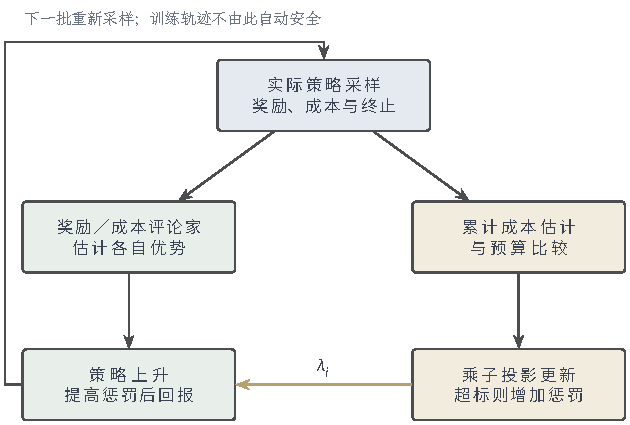
\includegraphics[width=106.659mm]{figures/10-reinforcement-learning/03-task-expansion-and-trustworthiness/tikz/rl-trustworthy-primal-dual.pdf}
  \caption{期望成本约束的两条反馈。奖励与成本优势共同推动策略更新，累计成本与预算的差推动乘子更新；这是一种求解循环，不是每次采样均满足约束的证书。}
  \label{fig:rl-trustworthy-primal-dual}
\end{figure}

\begin{theorem}[有限折扣CMDP的强对偶]
  \label{thm:rl-trustworthy-strong-duality}
  固定有限状态集、各状态非空有限动作集、转移核$T$和初态分布$\mu_0$，取$0\leq\gamma<1$。奖励$R(s,a)$、非负成本$c_i(s,a)$及有限预算$b_i$均固定且有界，$J$和$J_{c_i}$为从$\mu_0$启动的未归一化折扣期望。至少有一个满足全部预算的策略时，允许随机平稳策略的CMDP与占用度量线性规划等价，且
  \[
    \begin{aligned}
      \max_{\pi:\,J_{c_i}(\pi)\leq b_i}J(\pi)
        &=\min_{\bm{\lambda}\geq0}g(\bm{\lambda}),\\
      g(\bm{\lambda})
        &=\sum_i\lambda_i b_i+
          \max_\pi\left\{J(\pi)-\sum_i\lambda_iJ_{c_i}(\pi)\right\}.
    \end{aligned}
  \]
  原始最优解和有限维线性规划的对偶最优解存在。
\end{theorem}

证明以式~\eqref{eq:rl-trustworthy-cmdp-lp}~的占用量替代策略。可行占用集是非空、有界、闭多面体，线性目标有有限最优值，有限维线性规划强对偶因而给出相等的原始与对偶最优值。流守恒对应状态价值变量，成本不等式对应非负乘子；保留成本乘子并对占用流最大化，就得到定理中的$g$。这里使用的是原始问题非空且最优值有限的有限维线性规划强对偶，用于核对CMDP目标与乘子目标是否等价；相关基础可参考\BookChapterRef{chap:optimization}{卷1《数学准备：计算、分析与几何》“最优化”章}。

互补松弛还要求
$\lambda_i^\star(J_{c_i}(\pi^\star)-b_i)=0$：预算严格富余时乘子必须为0，预算恰好用尽时乘子却未必严格为正。强对偶依赖占用多面体的线性结构，不依赖任意神经网络参数集的凸性。参数化策略可能表示不了最优占用量，交替梯度也可能停在非全局解，因此上述定理不能直接当作神经网络训练的收敛保证。

乘子通过惩罚间接推动成本达标，\term{约束策略优化}（constrained policy optimization, CPO）则在旧策略附近直接限制一次更新的成本代理。代理沿用旧策略的状态分布，候选策略实际运行后却有新的状态分布，因此还需控制两者之差。令旧策略$\pi$与候选策略$\pi'$均为平稳Markov策略，对奖励或任一成本$f$定义
\[
  \begin{aligned}
    S_f(\pi',\pi)
      &=J_f(\pi)+\frac{1}{1-\gamma}
          \mathbb E_{s\sim d^\pi,a\sim\pi'}A_f^\pi(s,a),\\
    \epsilon_f
      &=\max_s\left|\mathbb E_{a\sim\pi'}A_f^\pi(s,a)\right|.
  \end{aligned}
\]
在共同MDP、共同初态和有界优势下，有
\begin{align}
  J(\pi')&\geq S_r(\pi',\pi)
      -\frac{2\gamma\epsilon_r}{(1-\gamma)^2}\overline D_{\mathrm{TV}},
      \nonumber\\
  J_{c_i}(\pi')&\leq S_{c_i}(\pi',\pi)
      +\frac{2\gamma\epsilon_{c_i}}{(1-\gamma)^2}\overline D_{\mathrm{TV}},
  \label{eq:rl-trustworthy-cpo-bound}\\
  \overline D_{\mathrm{TV}}
    &=\mathbb E_{s\sim d^\pi}
          \frac12\sum_a|\pi'(a\mid s)-\pi(a\mid s)|. \nonumber
\end{align}
式~\eqref{eq:rl-trustworthy-cpo-bound}~给回报下界和成本上界，方向不同，是因为收益需要不太低、成本需要不太高。其关键是占用变化界
$\|d^{\pi'}-d^\pi\|_1\leq
2\gamma\overline D_{\mathrm{TV}}/(1-\gamma)$。
性能差恒等式原本在$d^{\pi'}$下平均优势；将其换成$d^\pi$，用$\epsilon_f$乘上占用差，再除以$1-\gamma$，就得到上述误差项。若
$\mathbb E_{d^\pi}D_{\mathrm{KL}}(\pi'\|\pi)\leq\kappa$，Pinsker不等式和Jensen不等式进一步给出
$\overline D_{\mathrm{TV}}\leq\sqrt{\kappa/2}$。因此，精确求得
$S_{c_i}$加上误差余量不超过$b_i$，才直接推出下一策略成本达标。完整的界与CPO构造见原论文\scite{rl8-achiam2017-cpo}

实际CPO以样本优势、成本约束的一阶近似和KL的二阶近似求局部步，再用线搜索检查代理量；通常也没有精确估计$\epsilon_f$的全状态上界。只让线性化成本代理低于预算，至多得到仍带余项的成本界，不能据此省略余项而宣称严格可行。

Lagrangian PPO或SAC将乘子惩罚接入各自策略目标，仍继承对应采样和近似误差；SAC若包含熵奖励，所优化回报还发生了改变。奖励约束策略优化（reward constrained policy optimization, RCPO）采用便于学习的替代惩罚与多时间尺度更新，其收敛依赖替代惩罚和原约束的关系、步长及优化假设。任意换一个奖励，并不能由此推出原成本约束达标\scite{rl8-tessler2019-rcpo}

只有离线日志、不能继续试错时，乘子更新还面临另一项困难：候选策略改变状态访问分布，而原日志中的成本均值未必是候选策略的成本。COptiDICE（Offline Constrained Reinforcement Learning via Stationary Distribution Correction Estimation）沿用第~\ref{chap:rl-information}~章DICE的占用流校正，将固定策略评价扩展为带成本约束的占用优化。为看清其接口，仍取有限状态动作、时间不变MDP、$0\leq\gamma<1$、固定初态$\mu_0$及有界奖励和非负成本。日志训练样本$D$包含状态、动作、奖励、各项成本与下一状态，另需与目标启动条件相符的初态样本；令$d_D(s,a)$表示日志转移记录的状态动作抽样分布。它可以来自多种行为机制的混合，不要求已知某个单一行为策略$\beta(a\mid s)$。

把候选归一化占用写成$d(s,a)=d_D(s,a)w(s,a)$，其中$w\geq0$。与式~\eqref{eq:rl-information-dice}~评价固定目标策略不同，此处策略也待求解，因此先匹配状态流：对每个状态测试函数$v:S\to\mathbb R$，理想总体约束为
\begin{equation}
 \mathbb E_{(s,a)\sim d_D,\,s'\sim T(\cdot\mid s,a)}
   \left[w(s,a)\{v(s)-\gamma v(s')\}\right]
   =(1-\gamma)\mathbb E_{s_0\sim\mu_0}v(s_0).
 \label{eq:rl-trustworthy-coptidice-flow}
\end{equation}
全部$v$的约束对应式~\eqref{eq:rl-trustworthy-cmdp-lp}~的状态流守恒，使加权后的记录可解释为某个候选策略的折扣访问，而非任意提高高奖励样本的权重。方法在归一化奖励目标$\mathbb E_{d_D}[wR]$中减去$\eta\mathbb E_{d_D}f(w)$，其中$\eta>0$，$f$为满足$f(1)=0$的严格凸可微函数，以惩罚占用量过度偏离日志分布；成本约束配非负乘子，状态流配状态势函数，经对偶化用转移样本学习$w$。这一占用正则化会改变无正则CMDP的优化目标，不能将两者的最优回报直接等同。

只代入经验均值$\mathbb E_{d_D}[wc_i]$仍可能低估成本。COptiDICE进一步对成本作稳健的上侧估计：将初态样本与$(s,a,s')$转移记录组成的联合样本律作为扰动对象，限制其相对经验联合律的KL距离不超过$\epsilon_{\mathrm{rob}}\geq0$，并要求扰动后的初始分布、转移条件律及$\widetilde p(s,a)w(s,a)$仍满足同一占用流方程。随后求这些兼容分布下加权成本$\mathbb E_{\widetilde p}[wc_i]$的上确界，再将上侧估计经非负乘子接入策略优化。原论文的对偶成本目标因此含状态势函数的流残差修正，不能替换为只对状态动作边缘分布任取KL球的$\mathbb E[wc_i]$。$\eta$控制占用正则强度，$\epsilon_{\mathrm{rob}}$控制成本扰动范围，两者具有不同作用。由于这里$J_{c_i}$未归一化，归一化占用下的成本上侧估计应与$(1-\gamma)b_i$比较，不能直接与$b_i$比较\scite{rl8-lee2022coptidice}

获得满足相应流约束的占用比后，有限动作情形可按
\begin{equation}
 \pi_w(a\mid s)=
   \frac{d_D(s,a)w(s,a)}
        {\sum_{a'\in\mathsf A(s)}d_D(s,a')w(s,a')},
 \qquad \sum_{a'}d_D(s,a')w(s,a')>0
 \label{eq:rl-trustworthy-coptidice-policy}
\end{equation}
恢复候选策略。式~\eqref{eq:rl-trustworthy-coptidice-policy}~归一化的是日志状态动作质量乘占用比，不是要求先恢复原行为概率。例如只有一个自循环状态、两个动作$L,R$、初态就在该状态时，取$d_D=(3/4,1/4)$和$w=(1/3,3)$，得到候选占用$(1/4,3/4)$，其总质量为1，满足任意$0\leq\gamma<1$下的状态流；恢复的动作概率也为$(1/4,3/4)$。这是抽取步骤的手算示例，不是算法在某个基准上学得的结果。连续动作通常用$\mathbb E_{d_D}[w\log\pi_{\bm\theta}(a\mid s)]$作加权行为克隆，所提取策略还会增加函数逼近与拟合误差。

原总体推导以日志分布充分支持为条件；支持不全时只能在已覆盖的经验CMDP中求解。分母为0的状态可另选合法策略，但日志没有据此识别这些选择的回报或成本；$d_D(s,a)=0$处也不能靠有限权重创造正占用。还须存在受日志支持且满足所选成本稳健约束的候选方案，否则惩罚和乘子都不能创造缺失的可行策略。在精确求解相应稳健问题时，成本上界针对所声明的联合扰动集；真实运行律是否被该集合覆盖须另有依据，KL半径本身不构成普遍的有限样本安全保证。采样、流匹配函数类、比率优化与策略抽取误差仍需核查，最终固定策略的成本也仍须按第~\ref{sec:rl-trustworthy-inference}~节的评价协议取证。

理想占用规划的全局最优与强对偶、近似更新的误差控制、最终策略的原成本验证，至此已有各自依据。它们仍未约束每条训练轨迹：即使输出策略平均成本达标，先前探索也可能违反安全要求。要约束整个学习过程，还须明确其事件或硬安全标准。

% Outline: 8.4.2
\subsection{轨迹事件概率约束下的安全学习}
\label{sec:rl-trustworthy-chance}

第二类约束直接盯住“出事”这件事本身，而不是出事造成的平均成本。如果要求直接限制整次导航出事的可能性，平均碰撞成本就不是所需指标。例如规格要求发生任意碰撞的概率不超过1\%。设$E_t$为动作$t$导致碰撞的事件，定义
\[
  F_H=\bigcup_{t=0}^{H-1}E_t,\qquad
  \mathbb P_\pi(F_H)\leq\varepsilon.
\]
这就是\term{机会约束}（chance constraint）：允许违约发生，但指定事件的概率须不超过阈值。阈值来自任务要求，时域$H$决定哪些动作纳入事件。$\mathbf1\{F_H\}$不区分一次与多次碰撞，也不区分损坏1个与100个部件，因此相同失败概率仍可能对应不同事故成本。

首次碰撞之后再次碰撞，不应重复计入“至少发生一次”的概率。为保存这段历史，把失败标记加入状态：令$z_0=0$、$z_t\in\{0,1\}$，并递推
$z_{t+1}=z_t\lor\mathbf1\{E_t\}$。若原系统和碰撞判定在状态、动作与后继状态上是马尔可夫的，则$(s_t,z_t)$也是马尔可夫状态，且
$\mathbb P_\pi(F_H)=\mathbb E_\pi z_H$。
对于以状态集合$\mathcal B$表示的危险区域，也可令$z_0=\mathbf1\{s_0\in\mathcal B\}$，将初始失败纳入事件；两种起始约定不能混用。

固定时间相关策略$\pi_t$后，从终端标记向前求期望，即可得到概率价值$v_t(s,z)$：
\begin{align}
  v_H(s,z)&=z,\nonumber\\
  v_t(s,z)&=\sum_a\pi_t(a\mid s,z)
       \sum_{s'}T(s'\mid s,a)
         v_{t+1}\bigl(s',z\lor e(s,a,s')\bigr),
  \label{eq:rl-trustworthy-probability-value}
\end{align}
其中$e(s,a,s')$为本步事件指示量。按$t=H-1,\ldots,0$回传，最后对$\mu_0$平均$v_0(s,0)$，就得到整回合失败概率；若计入初始危险状态，则改为平均$v_0(s,z_0(s))$。这里求的是事件概率，不是折扣回报，因此不应额外乘奖励任务的折扣因子。在$z_0=0$的约定下，也可定义首次失败成本
$k_t=\mathbf1\{z_t=0,z_{t+1}=1\}$，则$\sum_tk_t=z_H$；普通碰撞次数之和一般不等于$z_H$。

把单步要求接成回合要求，只需同一概率空间上的事件关系。取正整数时域$H$和任意可测事件$E_0,\ldots,E_{H-1}$，并集界给出
\[
 \mathbb P(F_H)=\mathbb P\left(\bigcup_{t=0}^{H-1}E_t\right)
 \leq\sum_{t=0}^{H-1}\mathbb P(E_t).
\]
因此，非负预算若满足$\mathbb P(E_t)\leq\varepsilon_t$且$\sum_t\varepsilon_t\leq\varepsilon$，就支持整回合失败概率不超过$\varepsilon$。这个结论不要求各步事件独立，用途是把可检查的单步概率预算接到回合事件；相关概率工具可参考\BookChapterRef{chap:random-variables}{卷2《数学准备：概率、因果与决策》的“随机变量与概率基础”章}。

并集界将各步事件概率相加，一条轨迹上的多次碰撞可能被重复计入，所以界可能保守。若预算针对尚未失败时的下一步，则应改用存活条件。令
$S_t=\bigcap_{j<t}E_j^c$，在$\mathbb P(S_t)>0$时定义
$q_t=\mathbb P(E_t\mid S_t)$，则由条件概率乘法
\[
  \mathbb P(F_H)=1-\mathbb P(S_H)
       =1-\prod_{t=0}^{H-1}(1-q_t).
\]
取条件预算$\beta_t\in[0,1]$，则$q_t\leq\beta_t$推出
$\mathbb P(F_H)\leq1-\prod_t(1-\beta_t)\leq\sum_t\beta_t$。
乘积来自连续存活的条件概率链，不来自事件独立性。$q_t$已对所有存活历史求平均；要求每个存活历史下的条件概率都不超过$\beta_t$，是更强的充分条件。某时刻存活概率若为0，整回合失败概率已经是1，无须再定义后续条件概率。因此，无条件$\mathbb P(E_t)$、存活条件$q_t$和特定状态下的概率，不能共用同一预算解释。

教学计算中，若每步给定存活后的碰撞概率都是0.01，则$H=10$时整回合概率为
$1-0.99^{10}\approx0.0956$，$H=100$时为
$1-0.99^{100}\approx0.6340$。这两个数不需要额外假设各$E_t$独立，因为条件概率已被直接给定。若要求100步整回合不超过0.01，并且均匀分配条件预算，每步应满足
$\beta\leq1-0.99^{1/100}\approx0.00010050$。
图~\ref{fig:rl-trustworthy-events}~另将多个训练回合括在一起：最终策略单回合的$F_H$与训练期间任一回合出事的事件，具有不同样本空间和时域。

\begin{figure}[htbp]
  \centering
  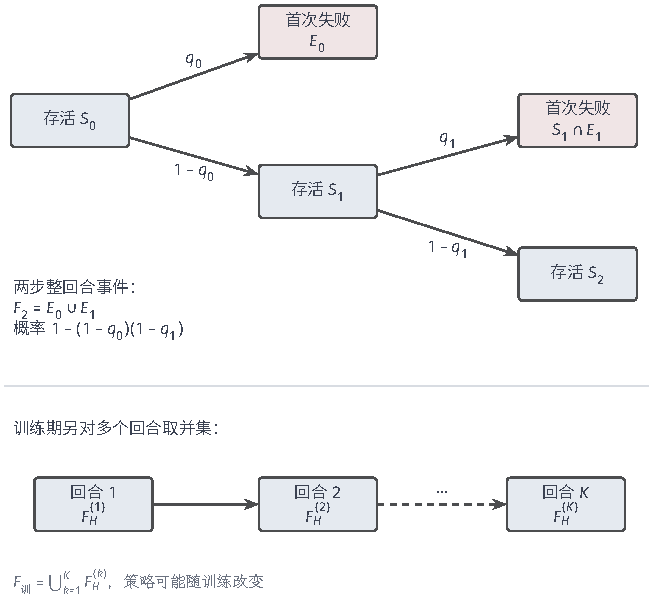
\includegraphics[width=110.652mm]{figures/10-reinforcement-learning/03-task-expansion-and-trustworthiness/tikz/rl-trustworthy-events.pdf}
  \caption{单步事件、整回合事件与整个学习过程事件。树在首次失败后合并成终止分支；下方回合可以使用不同策略，不能直接套用固定策略独立同分布的频率模型。}
  \label{fig:rl-trustworthy-events}
\end{figure}

事件定义明确后，学习方法取决于能否取得模型。直接采样时，每回合记录一次$z_H$，以均值估计概率，再用轨迹得分
$z_H\sum_t\nabla\log\pi(a_t\mid I_t)$估计概率梯度，并据此作拉格朗日约束更新。稀有事件使失败概率的相对误差更难控制，概率梯度也可能主要由极少数失败回合贡献；一批全为零的事件标记会使这份样本的梯度估计为0，但这只是没有观测到失败，不是安全证明。

模型已知时，可由式~\eqref{eq:rl-trustworthy-probability-value}~评价候选，或在时间和失败标记增广状态上优化期望终端成本，单次稠密评价代价为$O(H|S|^2|\mathsf A|)$。两种方法都需要完整事件标记；超时截断后未记录的事故，不能被当作没有发生。

如果不同后继状态需要不同风险余量，还可将剩余允许概率作为决策状态。到达尚未失败的$(t,s)$，剩余预算为$b\in[0,1]$，候选动作$a$的立即失败概率为$p_f(s,a)$，即对$e(s,a,s')=1$的后继转移概率求和。给未失败后继分配$b(s')\in[0,1]$，用全概率将立即失败和未来失败分开：
\begin{equation}
  p_f(s,a)+
    \sum_{s':\,e(s,a,s')=0}T(s'\mid s,a)b(s')\leq b.
  \label{eq:rl-trustworthy-risk-budget}
\end{equation}
\begin{samepage}
一个两分支计算可以说明后继预算的含义。设动作以0.1概率立即失败，以0.3和0.6概率分别到达两个安全后继$s_1,s_2$，这三项概率之和为1。给后继分配$b(s_1)=0.2$、$b(s_2)=0.05$，若两个后继的后续策略分别保证失败概率不超过这些预算，则整个后续失败概率的上界为
\[
  0.1+0.3\times0.2+0.6\times0.05=0.19.
\]
当前预算$b=0.2$时，这项分配通过当前一步的预算检验；整体可行还要求两个后继预算均可实现。到达$s_1$后，0.2是条件于已经到达该状态且此前未失败的后续概率上限；到达$s_2$后，相应上限为0.05。二者先经到达概率加权，才与立即失败概率一起接受当前预算检验，因此不能都用$0.2-0.1$作为同一个“剩余概率”。
\par
\end{samepage}

式\eqref{eq:rl-trustworthy-risk-budget}右侧的$b$限制的是条件于当前尚未失败状态的整个后续失败概率。选择满足该式且未来回报最高的动作与预算分配，到达$s'$后携带$b(s')$继续；最后一步后未来失败概率为0，向后归纳即可证明总概率不超过$b$。随机化动作时，还须对动作取平均并保留选定分支的预算。连续预算增加状态维度，网格化则带来规模和近似误差；随意从$b$减去一个“风险分数”没有对应的概率依据。

直接处理事件概率困难时，可以考虑CVaR的保守替代，但需要让损失编码与失败事件对应。令$X(\tau)>0$恰好表示失败，例如轨迹上最大的边界超出量。$X$可积时，有
\[
  \operatorname{CVaR}_{1-\varepsilon}(X)\leq0
  \quad\Longrightarrow\quad
  \operatorname{VaR}_{1-\varepsilon}(X)\leq0
  \quad\Longrightarrow\quad
  \mathbb P(X>0)\leq\varepsilon.
\]
第一个箭头依据尾部均值不小于分位点，第二个依据分位点定义；CVaR因而同时约束尾部严重程度，通常比原事件要求更强。反向不成立：以0.99概率取$X=-1$、以0.01概率取$X=100$，满足$\varepsilon=0.05$的机会约束，但最差5\%均值为
$(0.01\times100-0.04)/0.05=19.2>0$。若直接令$X=\mathbf1\{F_H\}$，则
$\operatorname{CVaR}_{1-\varepsilon}(X)=\min(1,p/\varepsilon)$；
把这一非负量限制为0，要求的是$p=0$，远强于原机会约束。采用替代目标前，须检查损失编码是否保留了所需事件含义，不能只匹配CVaR的名称和分位水平。

表~\ref{tab:rl-trustworthy-chance-methods}~将所需模型或记录与方法对应：完整回合支持直接采样，可信模型支持概率递推和预算分配，违约量的尾部分布支持CVaR替代。选择的既是求解手段，也可能是一个更保守的约束，因此须同时核对模型、采样条件和行为含义。

\begin{table}[htbp]
  \centering
  \begin{tabularx}{\linewidth}{@{}>{\raggedright\arraybackslash}p{21mm}XX@{}}
    \toprule
    方法 & 所需模型与记录 & 计算及主要边界 \\
    \midrule
    整回合采样 & 完整事件标记、固定时域与初态协议 & 每回合一个Bernoulli量；罕见事件样本少 \\
    概率价值递推 & 转移模型、时间、已失败标记 & 逐阶段备份；模型漏掉危险转移即失效 \\
    风险预算分配 & 上述模型、剩余预算及后继分配 & 增广预算空间；可行分配未必存在 \\
    CVaR替代 & 可积违约量及其尾部分布 & 同时限制尾部严重程度；通常更保守 \\
    \bottomrule
  \end{tabularx}
  \caption{机会约束的四种处理方式。它们分别解决估计、规划或保守替代问题，不能用相同数值阈值互相替换。}
  \label{tab:rl-trustworthy-chance-methods}
\end{table}

\begin{samepage}
若学习过程有$K$回合，记第$k$回合失败事件为$F_H^{(k)}$，训练期事件是
$F_{\text{训}}=\bigcup_{k=1}^KF_H^{(k)}$。即使每个训练回合都有概率上界$\varepsilon_k$，也只能直接得到
$\mathbb P(F_{\text{训}})\leq\sum_k\varepsilon_k$；自适应训练中可先对过去训练历史给条件上界，再用全期望与并集界。仅验证训练结束后的策略，完全没有约束先前探索使用的策略序列。
\par
\end{samepage}

% Outline: 8.4.3
\subsection{逐步与逐轨迹硬要求下的安全学习}
\label{sec:rl-trustworthy-hard-safety}

逐步与逐轨迹硬要求直接排除声明范围内的违规行为。这时候逐时刻检查“当前是否合法”是不够的。若要求任何时刻都不越界，检查当前机器人位置仍合法还不够：高速逼近边界且制动力不足时，即使此刻仍在界内，下一步也可能已经没有任何安全动作。硬安全需要的是往前看一步，找到那些“进去之后还能一直安全待下去”的状态。对已知离散系统
$\bm{x}_{t+1}=f(\bm{x}_t,\bm{u}_t,\bm{w}_t)$，用任务规格定义允许状态集$\mathcal X$，用执行器能力定义输入集$\mathcal U(\bm{x})$，用运行协议或模型误差界定义扰动集$\mathcal W(\bm{x},\bm{u})$。

\begin{definition}[控制不变集与可恢复集]
  \label{def:rl-trustworthy-invariance}
  对已知离散动力学$\bm{x}_{t+1}=f(\bm{x}_t,\bm{u}_t,\bm{w}_t)$，固定允许状态集$\mathcal X$、各状态可执行输入集$\mathcal U(\bm{x})$及输入确定后的允许扰动集$\mathcal W(\bm{x},\bm{u})$。
  集合$\mathcal K\subseteq\mathcal X$是鲁棒控制不变的，如果每个$\bm{x}\in\mathcal K$都有输入$\bm{u}\in\mathcal U(\bm{x})$，使所有
  $\bm{w}\in\mathcal W(\bm{x},\bm{u})$对应的后继状态仍在$\mathcal K$。
  一个从$\mathcal K$内选择这类输入的规则称为备份策略。
  给定备份不变集和非负整数步数$N$，可恢复集由那些存在非预见控制策略、能在所有允许扰动下始终留在$\mathcal X$并于至多$N$步进入$\mathcal K$的状态组成；非预见指本步输入只能使用已观察历史，不能使用尚未发生的扰动。
\end{definition}

定义中的量词顺序是“存在同一个输入，使所有允许扰动都安全”，不是针对每个扰动事后另选输入。允许状态集未必满足这一条件，可恢复集也随输入限幅、扰动范围和可用时间改变。若还要求整条轨迹成本不超过$B$，须保留剩余预算
$b_{t+1}=b_t-c_t$、$b_0=B$，并在增广状态$(\bm{x}_t,b_t)$上要求$b_t\geq0$及未来可行。折扣预算对应扣减$\gamma^tc_t$，或采用一致的相对时刻预算递推；不能用期望成本评论家替代每条轨迹的余额。

\begin{theorem}[安全集的一步封闭性保证]
  \label{thm:rl-trustworthy-invariance}
  考虑离散系统
  \[
    \bm{x}_{t+1}=f(\bm{x}_t,\bm{u}_t,\bm{w}_t).
  \]
  固定集合$\mathcal K\subseteq\mathcal X$、可执行输入集$\mathcal U(\bm{x})$和允许扰动集$\mathcal W(\bm{x},\bm{u})$。假定动力学$f$已知，实际状态可准确获得，初态$\bm{x}_0\in\mathcal K$，实际扰动始终在声明集合内。若每个$\bm{x}\in\mathcal K$的可行保护输入集合
  \[
    \begin{aligned}
      \mathcal U_{\mathcal K}(\bm{x})
        =\bigl\{\bm{u}\in\mathcal U(\bm{x}):\ &
          f(\bm{x},\bm{u},\bm{w})\in\mathcal K,\\
        &\text{对所有 }\bm{w}\in\mathcal W(\bm{x},\bm{u})\bigr\}
    \end{aligned}
  \]
  非空，且执行器在每步实际施加其中一个输入，则每条允许扰动轨迹都满足$\bm{x}_t\in\mathcal K$，$t\geq0$。
\end{theorem}
\begin{proof}
  固定任意满足扰动集合限制的轨迹。初始条件给出$\bm{x}_0\in\mathcal K$，这是归纳起点。
  假设在某个$t$有$\bm{x}_t\in\mathcal K$。集合非空保证能够选择
  $\bm{u}_t\in\mathcal U_{\mathcal K}(\bm{x}_t)$；按定义，对所有允许扰动，特别是实际发生的$\bm{w}_t$，
  \[
    \bm{x}_{t+1}=f(\bm{x}_t,\bm{u}_t,\bm{w}_t)\in\mathcal K.
  \]
  归纳步成立，故所有有限$t$都有$\bm{x}_t\in\mathcal K$。由于起初固定的轨迹任意，结论对每条允许扰动轨迹均成立。
\end{proof}

归纳证明把每步的全称保持条件传到整条轨迹，因此每项前提都影响结论。$\mathcal U_{\mathcal K}$若为空，就不存在满足要求的保护输入；状态判断若有误，所选动作可能不属于真实状态的可行集合；扰动越界或未建模延迟也会破坏一步封闭性。状态只能估计为集合$\widehat{\mathcal X}_t$时，须让同一个输入对全部可能真实状态和允许扰动有效，并另行保证真实状态确实在估计集合内。

定理~\ref{thm:rl-trustworthy-invariance}~也给出了执行检查：先有已验证不变集$\mathcal K$，再检查候选输入是否使全部允许后继仍在$\mathcal K$内。这样的数学条件及其成立依据称为\term{安全证书}（safety certificate），也就是可据以检验行为的证明条件。算法~\ref{alg:rl-trustworthy-filter}~使用这一不变集证书；屏障函数和预测过滤器则提供构造或检验保持条件的其他方式。距离最小的修正只用于尽量保留候选意图，并不产生安全性；只有保护输入集合非空且距离最小值取到时，算法才能要求最近点。若最小值不取到或求解器未在时限内返回经验证的可行点，只能改用当前仍满足同一保持条件的备份；集合为空或备份也未通过当前检查时，须报告保证失效。

\begin{algorithm}[带可行性检查的安全过滤]
  \label{alg:rl-trustworthy-filter}
  \begin{algorithmic}[1]
    \Require 候选策略、有效状态估计集合、动力学及误差集合、已验证不变集$\mathcal K$及其一步保持条件、可用备份
    \For{每个执行时刻$t$}
      \State 取得候选动作$\bm{u}^{\text{候}}_t$，更新状态估计集合
      \State 按定理~\ref{thm:rl-trustworthy-invariance}~构造保护输入集合：同一输入须使所有可能真实状态在所有允许扰动下的后继都留在$\mathcal K$
      \State 若候选动作在集合中，直接使用；否则，仅在最近点存在且求解器及时返回时使用距离最小的可行输入
      \State 若最近点不存在或优化超时，改用经过当前一步保持检查的备份；若集合为空或备份也不可行，报告保证失效并触发预设应急机制
      \State 执行实际动作，记录候选、实际动作、干预原因和后继状态，反馈给学习器
    \EndFor
  \end{algorithmic}
\end{algorithm}

过滤优化超时后，备份能否接管仍要在当前状态检查。应急停止只有满足相同模型和可行性条件时，才是证明中的安全输入；若已经没有安全制动距离，“优化失败就刹车”不能恢复已丢失的保证。图~\ref{fig:rl-trustworthy-filter}~因而将模型、状态估计和备份直接送入保护模块，并把实际动作反馈给学习器。

\begin{figure*}[t]
  \centering
  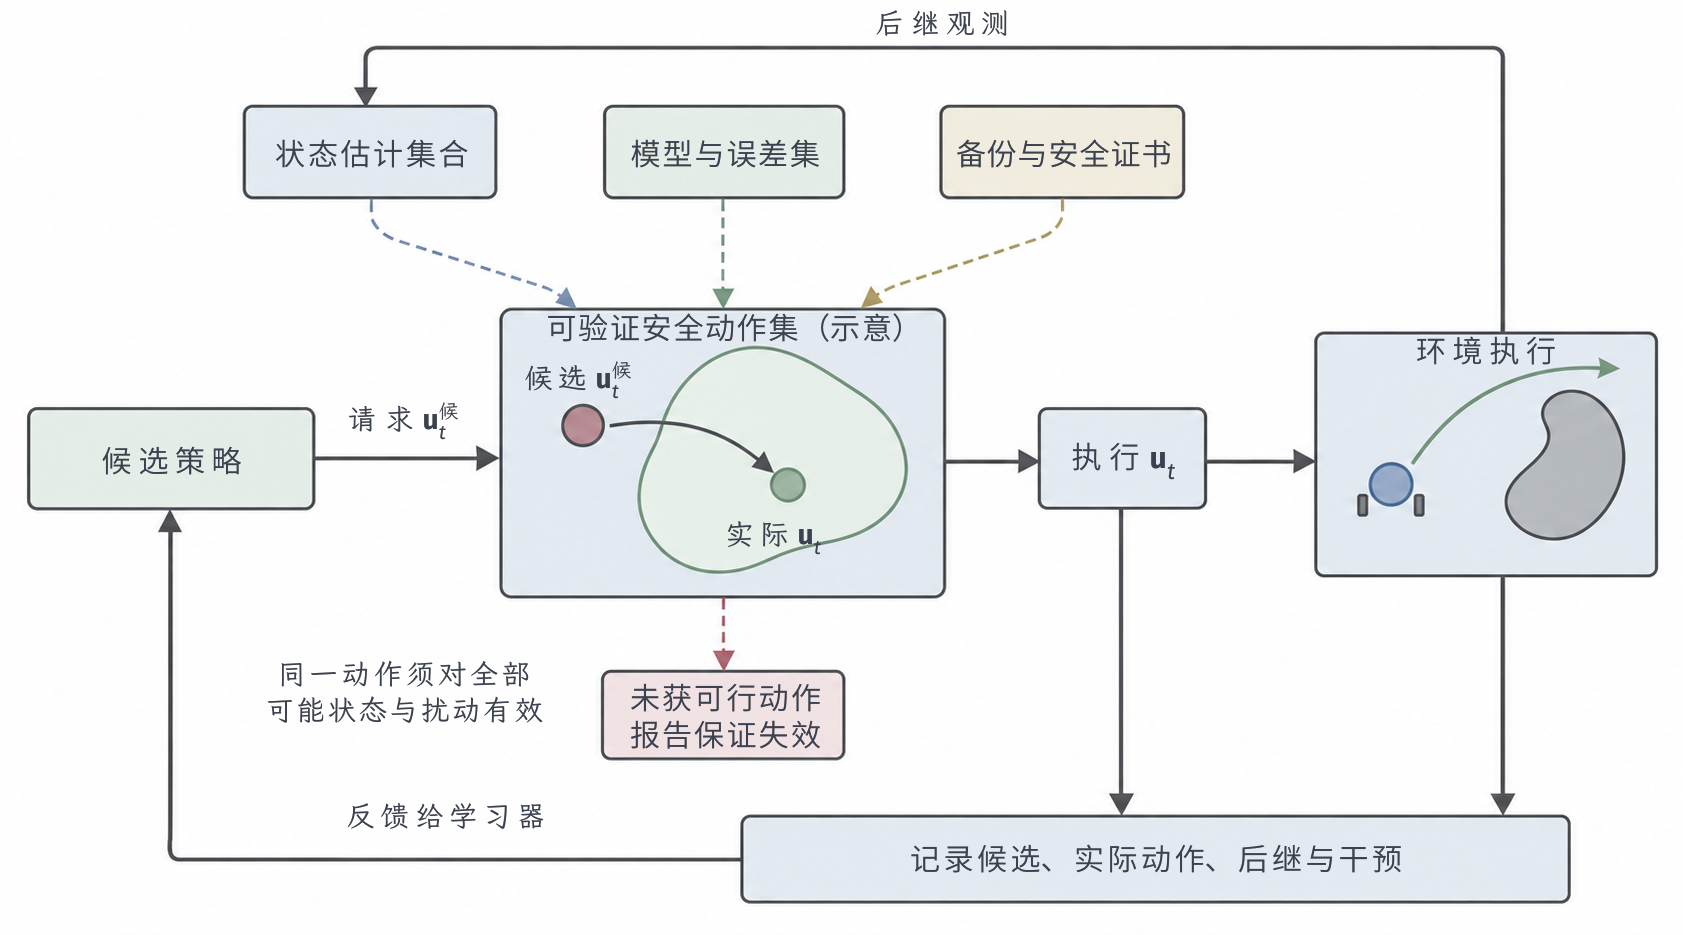
\includegraphics[width=157.400mm]{figures/10-reinforcement-learning/03-task-expansion-and-trustworthiness/generated/rl-trustworthy-filter/figure.png}
  \caption{保护器对控制动作的筛选与执行。实线连接候选动作、实际动作、环境和执行记录，虚线给出保护判断依赖的状态估计、模型与证书。动作区域仅为集合示意，不表示凸性、最近点存在或精确投影；未取得可验证动作时报告保证失效。右侧避障场景仅示意执行，评价仍须说明保护是否启用及保证针对哪个组合系统。}
  \label{fig:rl-trustworthy-filter}
\end{figure*}

离散动作下，可以屏蔽不满足一步保持条件的动作。若安全动作上的候选策略总质量为正，就将这些动作的原概率按该总质量归一化；若总质量为0，例如确定性候选只提出危险动作，则改用预先声明且经当前保持条件验证的备份分布。安全动作集为空，或备份分布不再受其支持时，屏蔽规则没有可执行的安全选择，必须报告保证失效。任务规格若含历史要求，屏蔽状态还可能包括表示规格进展的任务自动机或历史标记。普通\term{动作屏蔽}（action masking）只删除“向墙内移动”等即时非法动作，未必保留未来安全；按安全规格构造的屏蔽则在抽象模型上维护允许后继，其保证取决于抽象是否覆盖真实系统\scite{alshiekh2018shielding}

连续输入下，若可行集非空且最近点存在，可在其中找距离候选最近的动作，以尽量保留候选意图：
\[
  \min_{\bm{u}\in\mathcal U_{\mathcal K}(\bm{x})}
          \|\bm{u}-\bm{u}^{\text{候}}\|^2.
\]
教学系统$x_{t+1}=x_t+u_t+w_t$取$\mathcal K=[0,1]$、
$u_t\in[-0.2,0.2]$、$w_t\in[-0.05,0.05]$。鲁棒一步条件为
$0.05-x_t\leq u_t\leq0.95-x_t$。在$x_t=0.96$时，候选$u_t=0.1$会使最坏后继达到1.11；与输入限幅取交后，可行集为$[-0.2,-0.01]$，投影得到$u_t=-0.01$，后继范围为$[0.90,1.00]$。投影将朝边界的正动作改为负动作，是因为可行区间已计入最坏扰动；后继范围的显式计算才是保持安全的依据。

为了把“始终留在安全区”这一几何条件变成算法可以逐次检查的输入约束，\term{控制屏障函数}（control barrier function, CBF）用$h(\bm{x})\geq0$表示允许区域（状态安全当且仅当$h$非负），并限制输入使$h$不变为负。离散时间须检查
$h(f(\bm{x},\bm{u},\bm{w}))\geq0$对允许扰动成立，或者使用能够推出这一条件的更强不等式。连续时间控制仿射系统
$\dot{\bm{x}}=\bm{f}(\bm{x})+\bm{g}(\bm{x})\bm{u}$则常使用
\[
  \nabla h(\bm{x})^\top
       \bigl(\bm{f}(\bm{x})+\bm{g}(\bm{x})\bm{u}\bigr)
        \geq-\alpha_h(h(\bm{x})).
\]
其中$h$连续可微，$\alpha_h$是适当的扩展类$\mathcal K$函数，即连续、严格递增且$\alpha_h(0)=0$。不等式限制$h$下降的速度，使它在边界处不能继续朝负值方向穿越。在边界处$\nabla h\neq0$、声明时域内闭环解存在且唯一、输入约束下不等式始终可行、实际反馈满足不等式且初态在集合内等条件下，比较原理支持正向不变性，即闭环轨迹在声明时域内留在允许集合。它在此用于限制训练所得策略请求的动作；相关控制基础可参考\BookChapterRef{chap:policy-realization-and-control}{卷2《数学准备：概率、因果与决策》“策略的实现与轨迹控制”章}。

控制仿射性使输入以线性形式出现在约束中，常可和二次投影目标组成\term{二次规划}（quadratic program, QP）。输入饱和或多个约束冲突仍可能使QP不可行。连续时间不等式只约束所分析的连续闭环，采样间隔、执行延迟和模型误差还须通过余量或离散分析另行覆盖\scite{rl8-ames2017-barrier}

\term{预测安全过滤器}（predictive safety filter）把检查延伸到未来控制计划：预测时域内状态和输入都满足约束，末端进入已有备份能够维持的不变集，优化目标则可优先保留当前候选动作\scite{rl8-wabersich2021-filter}
鲁棒版本须使用反馈计划或误差管束；管束保存的是各步所有允许状态，而非一条标称避障轨迹。若执行一步后真实状态仍在旧的可行管束内，下一时刻就可向前平移旧计划，并在末端接上备份控制。这给出递归可行性的依据，即本次可行能为下一次留下可行方案。

误差集合突然扩大、终端集失效、状态估计离开管束或求解未按时完成，都可能破坏这一依据。预测步数、状态维度和非线性误差传播还决定在线代价，因此采用“MPC过滤”并不免除模型覆盖、可行性和求解时限的检查。

过滤维持当前可行性，恢复控制则把系统带回已验证区域，并须在返回过程中保持约束。停止学习任务、返回安全种子可以是整体方案的一部分。近期安全复位研究联合建模到达复位区域与避开危险；无人干预学习因此还要检查回合之间的重置，而不只检查单回合动作。这扩大了保证时域，也增加了复位路径、时间和控制能力的要求，不能假定复位天然安全或没有代价\scite{rl8-begzadic2025-reset}

上述过滤依赖动力学，模型未知时通常要从已知安全种子区域或备份控制开始，用保护器实际执行后取得的状态、实际动作及后继状态记录缩小模型误差集，再扩展可验证区域。高斯过程（Gaussian process, GP）可以预测均值与不确定区间；但证书需要真实动力学在声明状态输入范围及所有取证时刻上，以至少$1-\delta$的概率同时被模型集合覆盖。联合覆盖通常依赖函数正则性、噪声假设、置信参数及对自适应采样的控制。稳定性证书与GP误差界相结合的安全学习依赖这些条件，单有预测方差还不能支撑安全声明\scite{rl8-berkenkamp2017-safe}

记联合模型覆盖事件为$C_{\mathrm{cov}}$，结论可分两步表述：“在$C_{\mathrm{cov}}$上，过滤器按不变性条件保持安全；取证程序满足$\mathbb P(C_{\mathrm{cov}})\geq1-\delta$。”前一步是条件于模型覆盖的逻辑保证，后一步才是统计覆盖。单个点的95\%预测区间不能替代整条闭环轨迹的联合事件。扰动若有无界支持，也不能无条件假定所有时刻均在有界集合内；有限时域高概率覆盖与无限时域逐轨迹保证须分别论证。

多机器人共享狭窄通道时，两个机器人若都假定“对方会等待”，各自可能有可行计划，联合执行却会相撞。团队保证因而还须核对联合输入约束、通信延迟和参与者的建模承诺。去中心化过滤只有在局部假设相容、联合可行域非空且执行时可读取的观测、状态与消息符合证明条件时，才可能支持团队安全；个体QP各有一个解不够。参与者响应模型仍由第~\ref{chap:rl-multi-agent}~章提供。

% Outline: 8.5
\section{可靠性评价与保证}
\label{sec:rl-trustworthy-evidence}

前面几节解决的是“怎样求出一个试图满足要求的策略”，但求解器在训练中优化了某个代理目标，不等于交付对象真的满足原要求；受保护系统长期无事故，也可能只是保护器在起作用，无法说明移除保护后的表现。所以还需要一个独立于训练的取证环节：预先固定取证协议，再依据评价样本或模型证明，估计各项指标落在什么范围、保证覆盖到哪里。图~\ref{fig:rl-trustworthy-validation}~显示这一依赖：运行条件改变时，旧成功次数是否仍可使用，须先重新核对协议。

\begin{figure*}[t]
  \centering
  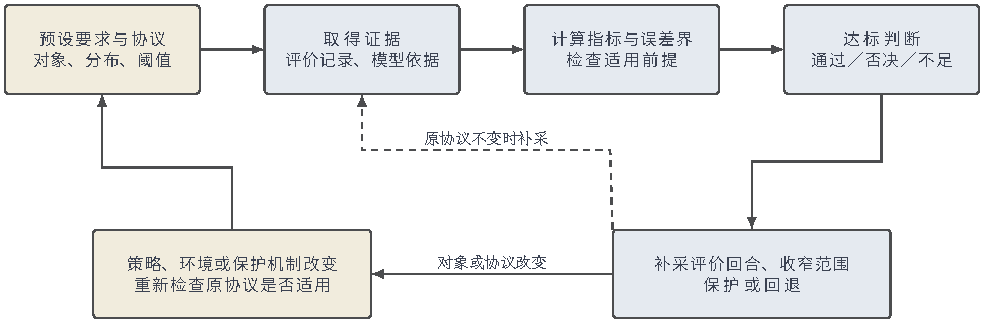
\includegraphics[width=166.617mm]{figures/10-reinforcement-learning/03-task-expansion-and-trustworthiness/tikz/rl-trustworthy-validation.pdf}
  \caption{运行记录、性能估计与可靠性判断之间的依赖。判断可以触发补充取证、收窄范围、保护或回退；原协议不变时，虚线返回允许补采记录。评价对象、保护配置或协议改变时，先重新核对协议，再取证和估计。流程本身不替代统计覆盖或模型证明。}
  \label{fig:rl-trustworthy-validation}
\end{figure*}

% Outline: 8.5.1
\subsection{确定验证协议并取得证据}
\label{sec:rl-trustworthy-protocol}

取证的第一步不是算统计量，而是把“这次运行到底在检验什么”固定下来。导航验证可以改变初始位置、训练种子或摩擦条件，但三种变化回答不同问题。固定策略从不同位置启动，评价其运行分布；换种子重新训练，评价学习规则产生的训练模型的变化；同一系统换摩擦条件，检查声明运行范围。未经区分就汇总成功率，会把策略、初态与环境三方面的影响混在一起，无法归因。

协议首先按保证对象冻结不同内容。评价固定策略或策略与保护层的组合时，冻结交付策略和保护器版本；评价固定学习规则的重复训练时，冻结训练流程、训练记录的生成与采样机制、训练样本预算、种子分布以及输出策略的验收规则，单次训练产生的输出策略本身是随机对象，不能事先冻结。随后再确定统计单位、初态与环境抽样分布、时域和终止规则、允许扰动与参与者、失败判定、回报与成本阈值及置信要求。这些约定决定怎样把一次运行或一次完整训练转成证据。碰撞若定义为“机身越过边界”，仅记录报警就不足以判定事件。恢复时间也须约定起点和恢复集合；观察结束仍未恢复，意味着真实恢复时间尚不完整，应按删失或超时规则处理，不能删去这些回合后计算平均值。

表~\ref{tab:rl-trustworthy-evidence-sources}~对应证据来源与可支持结论。模型证明覆盖显式模型的全部允许情况，运行试验则有助于发现实际系统中的模型遗漏。两者可以互补，但模型前提和试验抽样范围都须保留在结论中。

\begin{table*}[t]
  \centering
  \begin{tabularx}{\linewidth}{@{}>{\raggedright\arraybackslash}p{23mm}XXX@{}}
    \toprule
    证据来源 & 统计单位与可控条件 & 可支持结论 & 关键缺口 \\
    \midrule
    重复训练 & 一次完整训练；算法、预算、种子分布固定 & 输出策略指标分布、训练失败概率 & 不能只挑最好种子报告 \\
    固定策略重复运行 & 一回合；策略和运行协议冻结 & 协议分布下的回报、成本和事件概率 & 回合独立性、有效样本量 \\
    压力测试 & 指定极端场景或攻击；权限固定 & 已测条件下的失效及响应 & 不直接给常态运行失败频率 \\
    已有日志 & 日志中的回合；行为机制可追溯 & 覆盖与校正条件下的离线评价 & 漏报事件、选择性记录、支持不足 \\
    形式化模型分析 & 模型中的状态、轨迹或扰动集合 & 前提成立时的全称性质 & 真实系统是否满足抽象与误差前提 \\
    \bottomrule
  \end{tabularx}
  \caption{取证方式与保证对象的对应关系。重复训练的一条学习曲线不是一次固定策略运行，主动挑选的极端情况也不是从日常运行分布随机抽到的回合。}
  \label{tab:rl-trustworthy-evidence-sources}
\end{table*}

要避免选择偏差，最终检验使用的任务与运行记录也须与开发使用的任务及训练记录区分。任务、攻击和训练种子一旦用于更新策略，就不再是未使用的测试证据；验证集若用于反复挑选策略，也已参与选择。可以分开开发、策略选择和最终验收，或事先使用对整个候选类同时有效的界。只留出随机种子仍不够：困难地形若被反复用于调节保护阈值，这些地形上的运行反馈已经参与方案调整。对预先冻结的候选，独立评价样本支持相应的固定候选风险界；从同一批样本中选择候选时，须让界同时覆盖预定候选类，或在选择后另取独立评价样本。相关原则可参考\BookChapterRef{chap:trust-reliability}{卷3《基础、理论与可信性》“可靠性”章}。

为还原执行机制，每回合须保留初始条件、请求动作、实际动作、奖励、损失、成本、事件标记、接管时刻和恢复时间。失败后的运行记录有助于诊断后果和恢复，不应因回合“已经失败”而从日志消失。干预率还须固定分母：被替换动作占总动作的比例，和至少接管过一次的回合比例，衡量的是不同性质。

稀有事件的难点是有效危险样本少，复制成功轨迹不会增加独立的运行记录。重要性采样可以提高危险场景出现频率，但须知道目标运行分布相对采样分布的密度比、覆盖目标支持，并对完整事件统计加权。主动压力测试若没有这一密度比，只提供所测场景的证据。相关回合、长轨迹的重叠窗口或共享未重置环境状态的连续试验，也不能直接计作独立样本。

% Outline: 8.5.2
\subsection{由证据估计指标与保证范围}
\label{sec:rl-trustworthy-inference}

协议固定、评价记录收集完成后，下一步才是从有限样本估计指标，并说明这些估计可能偏出真实值多远。策略和协议冻结后，第$j$条完整轨迹给出$G_j,L_j,C_{i,j}$与失败标记$Y_j=\mathbf1\{F_H^{(j)}\}$。回报和成本可取样本均值，失败概率可取$\widehat p=n^{-1}\sum_jY_j$；尾部损失则需经验分位数或式~\eqref{eq:rl-trustworthy-cvar}~的样本目标。各统计量使用的轨迹函数与损失样本不同：CVaR主要依赖少量尾部质量，不能直接沿用回报均值的标准误；恢复时间则须纳入观察结束仍未恢复的回合。

由评价样本计算的点估计只是一个数。置信界控制推断程序的覆盖错误，模型误差界控制近似模型与真实系统的偏差，形式化性质则给出前提下的逻辑结论。三者不能互相替代。单回合内状态可以高度相关，只要回合独立，整回合失败标记仍可作Bernoulli分析；把每步当成独立回合，却会同时改变事件和有效样本量。

对预先冻结的策略、运行分布和失败事件，固定正整数样本量$n$。若完整回合的失败标记独立同分布为$\operatorname{Bernoulli}(p)$，取$0<\delta<1$，观察到零次失败时，精确二项单侧置信上界为
\[
 U_0(n,\delta)=1-\delta^{1/n}.
\]
这里用它判断完整运行记录能否支持部署失败概率阈值；它不证明$p=0$，也不覆盖根据已见评价记录选择样本量或策略的未经校正程序。相关保证与证据原则可参考\BookChapterRef{chap:trust-foundations}{卷3《基础、理论与可信性》“可信机器学习基础”章}。

覆盖性质可以按一个完整推断程序理解：零失败时返回$U_0$，出现失败时返回1。真实$p\leq U_0$时它从不漏盖，$p>U_0$时漏盖只能发生在零失败批次，概率为$(1-p)^n<\delta$，所以程序覆盖率至少为$1-\delta$。这是重复抽样程序的保证，不是关于固定$p$的后验概率。

这个上界可以检查零失败记录是否足以支持部署阈值。取$\delta=0.05$，100次零失败的95\%单侧上界约为0.029513，即2.95\%，还不能支持1\%阈值。令$1-\delta^{1/n}\leq\varepsilon$并解出样本量，得到事先应选择
\[
  n\geq
  \left\lceil\frac{\log\delta}{\log(1-\varepsilon)}\right\rceil.
\]
因此，1\%阈值至少需要299次，0.1\%阈值至少需要2995次。表~\ref{tab:rl-trustworthy-zero-failure}~列出公式计算值，不是机器人实验结果。成功回合较多与能够排除指定稀有失败水平，是不同结论。

\begin{table}[htbp]
  \centering
  \begin{tabular}{@{}rrl@{}}
    \toprule
    固定样本量$n$ & 95\%失败概率上界 & 与阈值比较 \\
    \midrule
    100  & 0.02951305 & 尚不能支持$p\leq0.01$ \\
    299  & 0.00996915 & 支持$p\leq0.01$ \\
    1000 & 0.00299125 & 尚不能支持$p\leq0.001$ \\
    2995 & 0.00099974 & 支持$p\leq0.001$ \\
    \bottomrule
  \end{tabular}
  \caption{零失败的解析教学上界。每行分别代表预先固定样本量的独立验证，不代表持续查看同一次试验并在达标时停止的程序。}
  \label{tab:rl-trustworthy-zero-failure}
\end{table}

如果不允许运行候选策略而只有日志，先要判断日志能否识别其风险。按第~\ref{chap:rl-information}~章的轨迹重要性采样，固定共同环境、初态与完整记录字段，设已知行为机制$\beta$覆盖目标$\pi$。动作有限或可数时，可用沿途动作点概率比
$W_j^\pi=\prod_{t=0}^{H-1}\pi(a_{j,t}\mid I_{j,t})/
\beta(a_{j,t}\mid I_{j,t})$。
连续动作则要求目标条件动作核相对行为条件动作核绝对连续，将每个因子改为前者相对后者的Radon--Nikodym导数，在已记录动作处求值；若使用密度比，还须声明共同支配测度。对能由完整记录计算、且在目标下可积的$G,C_i$，就有
$\mathbb E_\beta[W^\pi G]=J_H(\pi)$及
$\mathbb E_\beta[W^\pi C_i]=J_{c_i,H}(\pi)$。
权重将行为分布下的期望换成目标分布下的期望，失败事件同样可用$W^\pi Y$估计。动作覆盖还不等于日志完整：碰撞后结果若被删去，权重不能恢复缺失记录。隐藏混杂、执行通道变化或目标动作无支持，都可能使安全指标无法由日志识别。

要同时检验性能改进和成本达标，可以分别构造回报差下界与成本上界。设固定候选$\pi$和固定基线$\pi_b$共用$n$条独立同分布行为回合，两者轨迹分布都相对行为分布绝对连续，即目标可能轨迹在行为分布下也有支持；只覆盖候选不足以评价它与基线之差。定义
$Z_j=(W_j^\pi-W_j^{\pi_b})G_j$与
$X_{i,j}=W_j^\pi C_{i,j}$。若已知
$Z_j\in[z_-,z_+]$、$X_{i,j}\in[0,x_{i,+}]$几乎处处成立，则Hoeffding不等式给出
\begin{align}
  J_H(\pi)-J_H(\pi_b)
     &\geq \overline Z
        -(z_+-z_-)\sqrt{\frac{\log(1/\delta_r)}{2n}}
        =:\mathrm{LCB}_{\Delta J}, \nonumber\\
  J_{c_i,H}(\pi)
     &\leq \overline X_i
        +x_{i,+}\sqrt{\frac{\log(1/\delta_i)}{2n}}
        =:\mathrm{UCB}_{c_i}.
  \label{eq:rl-trustworthy-offline-joint}
\end{align}
换测度恒等式给出$\mathbb E Z$为回报差、$\mathbb E X_i$为候选成本，再对有界独立样本分别施加单侧浓缩不等式，即得到式~\eqref{eq:rl-trustworthy-offline-joint}~。此处独立单位是一回合完整可见记录，已知权重和累计量的界使所估变量有界，因而满足所用单侧集中界的抽样条件。回报差从均值减去余量，成本从均值加上余量，分别保留所需的不利方向。用并集界，所有声明同时成立的概率至少为
$1-\delta_r-\sum_i\delta_i$，无须各估计量相互独立。检验
$\mathrm{LCB}_{\Delta J}\geq-\epsilon_{\text{改进}}$与
$\mathrm{UCB}_{c_i}\leq b_i$，才分别支持“不比基线差太多”和“成本达标”。折扣无限时域评价还要补上截断余项。

这套界的强假设是权重和结果有已知界；长时域的乘积权重可能极大，置信区间也就可能宽到无法判断。截断权重能降低方差，却引入须另行控制的偏差；模型辅助估计则引入模型前提。

基线自举的安全策略改进（safe policy improvement with baseline bootstrapping, SPIBB）将支持不足区域的行为限制在基线附近，研究相应行为日志与模型假设下的期望回报改进。这里的“safe”针对相对基线的性能，不直接针对成本或碰撞概率：基线可能本就不安全，候选也可能以较高风险换取较高回报。行为安全仍需单独的成本或事件上界\scite{rl4-laroche2019-spibb}

候选$\pi$若由同一批评价样本选出，固定策略的式~\eqref{eq:rl-trustworthy-offline-joint}~就不能原样使用。可以对预先确定的有限候选集分配总错误预算，采用对策略类一致有效的界，或冻结最终策略后使用独立留出评价样本。日志中的动作若被保护器替换，权重分母须描述实际行为机制；目标也是受保护系统时，分子也须描述组合机制。只有概率比对应交付对象，估计才是在回答其性能和安全问题。

表~\ref{tab:rl-trustworthy-indicators}~汇总各指标的覆盖条件。回报、尾部、事件和恢复过程可以来自同一份日志，误差控制却须分别建立；不变性还需核对真实闭环是否满足证书前提，不能由日志均值代替。

\begin{table*}[t]
  \centering
  \begin{tabularx}{\linewidth}{@{}>{\raggedright\arraybackslash}p{19mm}XXXX@{}}
    \toprule
    指标或性质 & 估计／验证方法 & 覆盖条件 & 主要误差来源 & 保证对象 \\
    \midrule
    平均回报、成本 & 回合均值、离线校正与单侧界 & 固定策略和协议；独立或已处理相关性 & 抽样、截断、权重与模型偏差 & 指定策略的期望值 \\
    尾部损失、动态风险 & 累计损失的分位及CVaR估计；嵌套目标另需逐阶段条件估计 & 损失与尾部样本假设；动态目标还需条件分布覆盖 & 稀有样本、阈值估计、选择及递推误差 & 事先声明的累计或动态风险 \\
    失败概率 & 完整事件频率、二项或加权界 & 事件、时域、运行分布明确 & 漏报、相关回合、分布改变 & 固定执行系统的回合事件 \\
    恢复时间 & 完整或删失的恢复时间记录分析 & 恢复集合、起止和删失规则固定 & 超时删除、选择性接管 & 指定恢复机制 \\
    不变性 & 模型、误差集、可行性证明 & 真实闭环满足全部模型前提 & 状态估计、未建模执行与越界扰动 & 证书覆盖的保护系统 \\
    \bottomrule
  \end{tabularx}
  \caption{不同指标需要不同的误差控制。一个回报评论家准确，并不意味着碰撞概率或尾部损失已被准确估计。}
  \label{tab:rl-trustworthy-indicators}
\end{table*}

模型校准也需要明确分布：价值、后果分布和世界模型应在哪个策略诱导分布下接受检查？在训练轨迹经常访问的环境状态上预测准确，未必覆盖新策略频繁访问的边界状态；多个模型一致，也可能共同漏掉危险机制，所以集成分歧不自动构成置信界。形式化结论还须逐项核对真实动力学、状态估计、保护动作与执行器，不能只检查名义控制算法。

% Outline: 8.5.3
\subsection{依据要求作出判断并持续复核}
\label{sec:rl-trustworthy-decision}

有了带误差范围的指标界，还要按正确的方向与阈值比较，并如实区分“达标、不达标、证据不足”三种结论，而不是非黑即白地只看点估计。指标界得到后，应在不利方向与阈值比较。失败概率要求$p\leq\varepsilon$时，$U_p\leq\varepsilon$支持达标，$L_p>\varepsilon$支持不达标；区间跨阈值则现有样本尚不足以判断是否达标。回报要求$J\geq j_{\min}$时方向相反，$L_J\geq j_{\min}$支持达标，$U_J<j_{\min}$支持不达标。多项要求还须预先控制联合置信错误率，各项分别有95\%区间并不意味着整体仍有95\%覆盖。

图~\ref{fig:rl-trustworthy-intervals}~上半部分中，两组零失败评价记录的点估计都为0，但100次试验的上界仍高于1\%，299次的上界才低于1\%。下半部分只用示意区间展示回报应检查下界，没有对应实验。样本尚不足以判断是否达标时，可按新的预设方案补充证据，或收窄部署范围到已有覆盖的条件。此时尚不能确认达标，也没有证实不达标；直接批准原范围部署同样缺少依据。

\begin{figure*}[t]
  \centering
  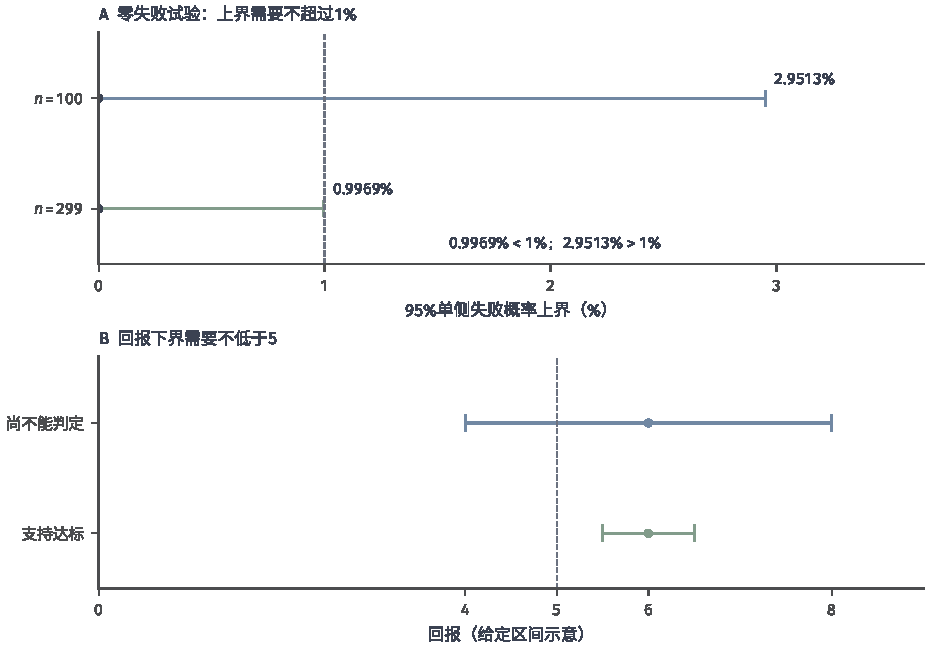
\includegraphics[width=157.400mm]{figures/10-reinforcement-learning/03-task-expansion-and-trustworthiness/matplotlib/rl-trustworthy-intervals.pdf}
  \caption{置信界与阈值的方向。上图按$n$次零失败的解析公式计算95\%单侧上界；下图仅以给定区间示意回报判断，不代表某个统计估计器或实验。点标估计，线段标可支持的指标范围。}
  \label{fig:rl-trustworthy-intervals}
\end{figure*}

达标判断还须绑定策略和协议版本。摩擦范围改变会影响轨迹分布，策略更新会影响状态动作占用，保护器升级会改变执行行为，参与者增加会改变闭环假设。旧运行记录未必全部失效，但须逐项说明哪些条件仍匹配、哪些运行记录需要重加权或补充、哪些模型性质须重新证明。交付对象或运行范围不再匹配时，旧安全声明不能直接沿用。

持续运行时，监测应检查保证前提：误差是否越出集合、备份是否仍可行、事件记录是否完整、干预比例是否明显改变。变化可触发保护、回退、收窄范围或补充取证，监测基础设施由系统卷讨论。统计判断也要覆盖查看方式：反复查看固定样本区间直到首次达标，并不自动保留原错误率。可预先为多次检验分配错误预算，或在相应评价记录的抽样条件下使用\term{置信序列}（confidence sequence），即对整个查看时间序列同时有效的界\scite{rl8-howard2021-sequences}

% Outline: 8.6
\section{多种要求的组合与取舍}
\label{sec:rl-trustworthy-combination}

三类要求至此分别讲完。为避免在不同任务上比较而让“任务本身的差异”掩盖“准则的差异”，现在把三类要求用于同一个导航选择。将基准网格抽象成单步路线选项任务：初态固定为起点，动作一次选择整段路线，结果给出到达终点总用时$T$、碰撞标记$I$和成本$C=10I$。这是独立教学模型，不使用基准网格的0.8滑移核；取$H=1$、不折扣、回报$G=-T$和损失$L=T$。路线内部的执行与恢复汇总为一次结果，时间以教学单位计。

候选集合先限定为四条确定路线A、B、C、D，所有比较固定同一初态和这组候选。干燥环境下，A以0.95概率用时5、以0.05概率用时25，B、C、D分别固定用时7、8、9。湿滑环境只将A、B用时各增加10，C、D不变。允许环境集合在本例中由这两个教学情形枚举给定，不是从观测记录估计的置信集。

两种环境中的碰撞概率依次为0.02、0.005、0.003、0。为分离时间与安全成本的影响，规定$I$和$T$独立，碰撞也不另外终止路线选项。这些假设共同确定联合分布，仅服务于控制变量比较，不是关于真实机器人碰撞与恢复的经验规律。

表~\ref{tab:rl-trustworthy-comparison}~据该联合分布精确计算。例如A平均用时为
$0.95\times5+0.05\times25=6$，0.95分位水平的CVaR为25，期望成本为$10\times0.02=0.2$，其余行用同样公式计算。回报越大越好，用时尾部、碰撞概率和成本越小越好。全部路线都关闭外部保护，干预为0；这只是固定执行机制，不是安全达标的证据。

\begin{table*}[t]
  \centering
  \begin{tabularx}{\linewidth}{@{}>{\raggedright\arraybackslash}p{14mm}XXXXXXX@{}}
    \toprule
    路线 & 标称平均回报 & 标称尾部损失 & 湿滑平均回报 & 碰撞概率 & 期望成本 & 干预比例 & 证据强度 \\
    \midrule
    A：捷径 & $-6$ & $25$ & $-16$ & $0.02$ & $0.20$ & $0$ & 教学模型精确值 \\
    B：定时 & $-7$ & $7$ & $-17$ & $0.005$ & $0.05$ & $0$ & 教学模型精确值 \\
    C：抗滑 & $-8$ & $8$ & $-8$ & $0.003$ & $0.03$ & $0$ & 教学模型精确值 \\
    D：保守 & $-9$ & $9$ & $-9$ & $0$ & $0$ & $0$ & 教学模型精确值 \\
    \bottomrule
  \end{tabularx}
  \caption{同一候选集合的解析教学比较。尾部损失为$\operatorname{CVaR}_{0.95}(T)$；碰撞概率和成本在两环境下按假设相同。D的零概率仅属于该指定模型，所有行均无真实部署统计证据。}
  \label{tab:rl-trustworthy-comparison}
\end{table*}

只最大化标称平均回报，会选A，却留下25的最差5\%平均用时。改为最小化标称尾部损失，选B，但其平均回报从干燥时的$-7$降到湿滑时的$-17$，回报减少10，也就是平均用时增加10。若最大化干燥与湿滑中的最坏平均回报，则选C；若仍优化标称均值，只增加期望成本预算$b=0.01$，四个确定候选中只有D可行。同一策略跨环境的下降幅度，还须与变化后的绝对值一起看：C、D的平均回报都没有下降，但变化后分别为$-8$与$-9$；若要求平均用时不超过8.5，C满足而D不满足。反过来，只看湿滑回报也无法区分原来就慢与湿滑额外造成的延误。这里的比较仍固定初态、候选和用时单位，每次求解只改一类要求，并非四个依次执行的算法阶段。

允许策略类若扩大到出发前随机选路线，结论还会变化。以0.2概率选B、0.8概率选D，期望成本为$0.2\times0.05=0.01$，平均用时为$0.2\times7+0.8\times9=8.6$，优于确定选D的9。因此D的上述最优性只针对四个确定候选，与示例~\ref{ex:rl-trustworthy-randomization}~相符。一次运行仍会完整选择B或D，不会走一条“平均路线”，B回合的碰撞可能也仍存在。

上面每次只施加一类要求。当它们同时出现时，不能简单地先按一个准则选策略、再指望它碰巧满足其余要求，而要把“在满足其余要求的策略中优化主目标”写成一个带约束的优化问题。这些要求若同时存在，须先由物理范围、枚举场景或观测记录给出的覆盖界确定模型族$\mathcal M$，再确定允许策略类$\Pi$。可以在保证最坏回报不太低、最坏成本不太高的前提下，最小化最坏风险：
\begin{align}
  \min_{\pi\in\Pi}\quad&
      \sup_{M\in\mathcal M}\mathcal R_M(L^\pi), \nonumber\\
  \text{满足}\quad&
      \inf_{M\in\mathcal M}J_M(\pi)\geq j_{\min}, \nonumber\\
  &\sup_{M\in\mathcal M}J_{c_i,M}(\pi)\leq b_i
       \quad (i=1,\ldots,m_c).
  \label{eq:rl-trustworthy-combined-problem}
\end{align}
这里$\mathcal R_M$须事先选为静态或动态风险，$\Pi$须说明历史依赖和随机化范围。风险与成本越大越差，故对模型取上确界；回报越小越差，故取下确界。这使每项要求分别覆盖全部允许模型。在路线例中，$\mathcal M$可以就是干燥与湿滑两情形；没有场景概率时，不能对二者作概率平均，即使给出概率，平均达标仍可能由干燥时的收益抵消湿滑时的违反，不能代替逐模型约束。只对回报作鲁棒优化，不会自动使成本鲁棒；鲁棒成本达标也不保证任务收益足够。

图~\ref{fig:rl-trustworthy-intersection}~将各项阈值对应的允许策略画成集合，最终可行域是这些集合与$\Pi$的交集。固定目标和策略类后，增加约束只能保持或缩小可行域，不会使最优值自动改善。在四个确定路线中，同时要求标称CVaR不超过8、最坏平均用时不超过9、期望成本不超过0.01，就没有可行选项：C满足前两项而成本超标，D满足后两项而尾部用时为9。此时须扩大策略类、改变环境或协商阈值；求解器返回的最少违反方案仍未满足原要求。

\begin{figure}[htbp]
  \centering
  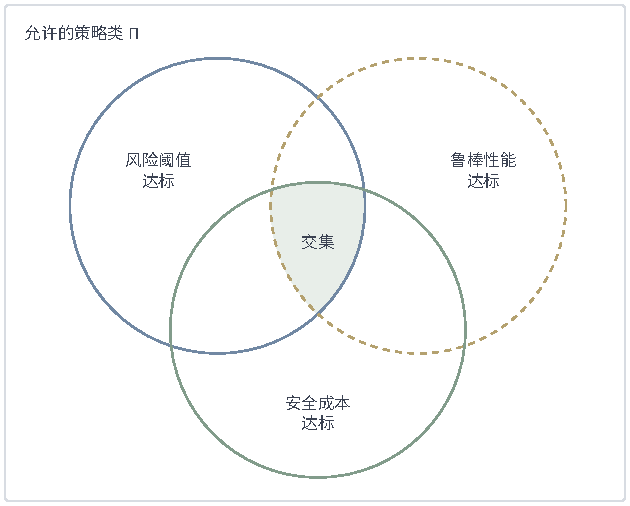
\includegraphics[width=106.652mm]{figures/10-reinforcement-learning/03-task-expansion-and-trustworthiness/tikz/rl-trustworthy-intersection.pdf}
  \caption{可行策略集合的概念示意，不是教学路线数值的几何嵌入。阴影为三种阈值共同允许的策略；在具体任务中，交集也可能为空。集合边界形状没有凸性含义。}
  \label{fig:rl-trustworthy-intersection}
\end{figure}

要识别保护器贡献，再固定同一候选，只切换保护是否启用。图~\ref{fig:rl-trustworthy-protected-path}~保留基准网格起终点和障碍，但采用无滑移的确定教学动力学，并将$(3,1)$规定为危险格。关闭保护，候选沿下方五步路径穿过危险格；启用保护，在$(2,1)$拒绝向右请求，转交已验证备份返回$(1,1)$，再沿上方到终点，共七步。该备份在这一确定模型中不进入障碍和危险格；恢复随机滑移后，须重新检查所有允许后继，原路径不能直接成为鲁棒安全证书。

\begin{figure}[htbp]
  \centering
  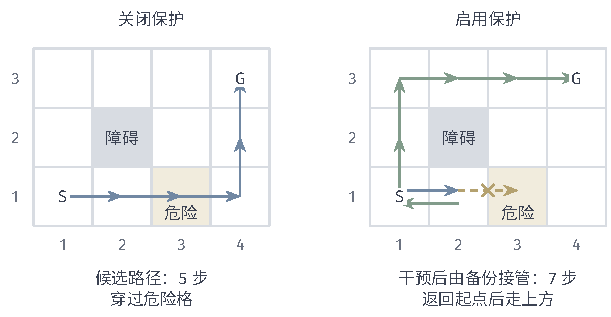
\includegraphics[width=103.470mm]{figures/10-reinforcement-learning/03-task-expansion-and-trustworthiness/tikz/rl-trustworthy-protected-path.pdf}
  \caption{同一候选启用或关闭保护的确定性路径示意，坐标、障碍和起终点沿用基准网格。虚线为被拒绝的请求，实线为实际路径；右图在干预后使用备份，不表示候选策略已自行学会绕行。}
  \label{fig:rl-trustworthy-protected-path}
\end{figure}

右图避免了一次危险格穿越，代价是两步额外行程和一次转入备份控制的切换。保持安全的是受保护系统，未保护候选仍请求经过危险格。图中一次拒绝也不等于全回合只替换一个动作，后续备份动作仍须由日志区分。保护改变了实际执行过程及其可见记录分布，学习器看到的安全轨迹可能来自外部修正；继续训练时须保留请求与实际动作，才能判断学到的是候选能力还是保护贡献。

这些比较同时呈现收益与代价。扩大不确定集合能增加覆盖范围，却可能降低可达到的回报；收紧尾部或安全阈值可能增加绕行与接管；加强保护能减少危险探索，却也会减少某些动作的观测，使其效果更难识别。因此方案结论需要同时声明行为标准、环境范围、执行机制与证据，单一平均分数不足以表达取舍。序贯决策的验证还须把其他已经明确的行为要求落实到实际策略、运行机制和评价记录，逐项规定可计算的指标、适用条件及证据。

% Outline: 8.7
\section{本章小结}
\label{sec:rl-trustworthy-summary}

导航例中，平均最快的路线未必尾部延误最小，尾部延误较小的路线未必耐受湿滑，耐受湿滑的路线又可能违反成本预算。风险准则比较随机后果，鲁棒要求覆盖允许环境，安全约束划定可行策略；三者可以组合，各自的评价目标、观测或环境模型要求及证明条件仍须分别保留。

\begin{table*}[htbp]
  \centering
  \begin{tabularx}{\linewidth}{@{}>{\raggedright\arraybackslash}p{22mm}XXX@{}}
    \toprule
    要求 & 决定性条件 & 方法 & 相应证据 \\
    \midrule
    控制累计尾部 & 损失、分位水平及事前承诺明确 & 静态CVaR采样更新、状态增广 & 尾部估计误差与留出轨迹 \\
    条件风险一致 & 条件映射及状态分量与递归目标匹配 & 嵌套风险Bellman更新 & 算子性质及条件风险估计 \\
    覆盖环境变化 & 扰动位置、扰动者可读字段与集合结构明确 & 鲁棒规划、受扰训练、状态估计 & 模型覆盖、内层误差与压力测试 \\
    平均成本达标 & 成本单位、初态、折扣及策略类明确 & 占用规划、原始--对偶与局部约束更新 & 最终策略的成本上界 \\
    事件概率达标 & 事件、时域、条件预算一致 & 事件采样、概率递推、预算分配 & 完整事件记录与有效概率上界 \\
    逐轨迹保持安全 & 误差范围有效、初态可行且保护输入存在 & 屏蔽、不变集、屏障与预测过滤 & 真实闭环符合证书全部前提 \\
    可靠地作出判断 & 交付对象、运行协议和取证程序固定 & 留出验证、联合置信与持续复核 & 界与阈值比较，并标明现有样本尚不足以判断达标 \\
    \bottomrule
  \end{tabularx}
  \caption{本章的要求、条件、方法与证据。算法的优化目标与交付时能够成立的保证是两件需要分别检查的事。}
  \label{tab:rl-trustworthy-summary}
\end{table*}

静态累计CVaR保留事前损失分布，嵌套风险逐层评价条件后果，状态增广与时间一致性要服务于对应目标。鲁棒备份须明确扰动作用于动力学、观测还是执行通道，并保存对手权限所需的状态；矩形性才使局部最坏选择组成合法模型。期望成本允许个别高成本轨迹，事件概率允许有限违约概率，硬要求则在声明范围内排除违约。乘子、概率预算和安全过滤据此维护不同性质。

表~\ref{tab:rl-trustworthy-summary}~对应每项要求的条件、方法与证据。方法的名称不足以判断可信性，还需确定它维护的性质、评价固定策略还是受保护系统、依赖哪些模型和记录采集前提，以及这些前提改变后哪些结论仍成立。



若日志支持不足或隐藏风险不可识别，需要回到第~\ref{chap:rl-information}~章的观测范围、日志字段与动作覆盖条件；若奖励没有表达真正意图，需要第~\ref{chap:rl-reward}~章的奖励分析。新任务识别与适应由第~\ref{chap:rl-transfer}~章讨论，其他参与者响应由第~\ref{chap:rl-multi-agent}~章提供模型。这些条件改变时，既要检查决策问题是否改变，也要复核原证据是否仍覆盖交付对象；求解结束本身并不构成可信性保证。
